% ----------------------------------------------------------------------
% Capítulo: Resultados
%
% Resultados obtidos a partir das análises feitas e dos modelos ajustados. Usar
% gráficos, tabelas e valores numéricos para ilustrar os achados. Cada
% figura e tabela deve ser referenciada no texto e possuir uma legenda
% concisa. As tabelas e figuras devem ser listadas automaticamente
% nas listas de tabelas e figuras.

\chapter{Resultados}


A Tabela \ref{tab:idade_gestacional_por_causa} apresenta a distribuição da idade 
gestacional ao parto (em semanas) segundo o desfecho da gestação. Entre os 
óbitos fetais (n = 3.268), a idade gestacional apresentou mediana de 29 semanas 
e intervalo interquartílico de 24 a 35 semanas. Como medida complementar, a média 
foi de 29,39 semanas (DP = 6,19). Em conjunto, esses valores mostram que uma parte importante dos 
óbitos fetais ocorreu em idades gestacionais mais precoces, desde o final do 
segundo trimestre até o terceiro trimestre da gestação, com variabilidade 
considerável no momento do desfecho. Os valores mínimo e máximo 
observados (3 e 43 semanas, respectivamente) indicam a presença de registros em 
semanas gestacionais extremas, mas, como atendem à definição de óbito fetal 
adotada, foram mantidos na análise.

Entre os nascimentos vivos (n = 485.922), a idade gestacional mostrou forte 
concentração em torno do termo, com mediana de 39 semanas e intervalo 
interquartílico de 38 a 39 semanas. A média foi de 38,26 semanas (DP = 2,13). Esses valores 
mostram baixa dispersão e reforçam que a maior parte das gestações com nascimento 
vivo chegou a uma idade gestacional adequada para o parto.

%---------------------- Tabela de medidas para idade gestacional
\begingroup
  \setlength{\tabcolsep}{2.5pt}
  \renewcommand{\arraystretch}{0.95}

  \begin{center}
    \begin{longtable}{%
      L{0.20\textwidth} % Causa (desfecho) - um pouco menor
      L{0.08\textwidth} % n                  (valores pequenos, pode ser estreita)
      L{0.06\textwidth} % Mín.               (abreviado)
      L{0.09\textwidth} % Média              (ganha espaço)
      L{0.09\textwidth} % Mediana            (ganha espaço)
      L{0.08\textwidth} % Q1
      L{0.08\textwidth} % Q3
      L{0.06\textwidth} % Máx.               (abreviado)
      L{0.08\textwidth} % DP
    }

    \caption{Medidas descritivas da idade gestacional (semanas) segundo o desfecho da gestação.}%
    \label{tab:idade_gestacional_por_causa}\\
    % Cabeçalho
    \toprule
    \textbf{Causa} &
    \textbf{n} &
    \textbf{Mín.} &
    \textbf{Média} &
    \textbf{Med.} &
    \textbf{Q1} &
    \textbf{Q3} &
    \textbf{Máx.} &
    \textbf{DP} \\
    \midrule
    \endfirsthead

    \caption[]{Medidas descritivas da idade gestacional (semanas) segundo o desfecho da
    gestação (continuação).}\\
    \toprule
    \textbf{Causa} &
    \textbf{n} &
    \textbf{Mín.} &
    \textbf{Média} &
    \textbf{Mediana} &
    \textbf{Q1} &
    \textbf{Q3} &
    \textbf{Máx.} &
    \textbf{DP} \\
    \midrule
    \endhead

    \midrule
    \multicolumn{9}{r}{\footnotesize Continuação na próxima página} \\
    \midrule
    \endfoot

    \bottomrule
    \endlastfoot
    % Corpo da tabela
    % Linha 1: Óbito fetal
    Óbito fetal &
    3\,268 &
    3 &
    29{,}39 &
    29 &
    24 &
    35 &
    43 &
    6{,}19 \\

    % Linha 2: Nascimento vivo
    Nascimento vivo &
    485\,922 &
    19 &
    38{,}26 &
    39 &
    38 &
    39 &
    45 &
    2{,}13 \\
    \end{longtable}
  \end{center}
\endgroup

A Figura \ref{fig:histograma_ambas_causas} reforça esse comportamento. Na mediana, 
os óbitos fetais ocorreram cerca de 10 semanas antes dos nascimentos vivos e ao 
longo de uma faixa mais ampla de idades gestacionais, mostrando maior 
variabilidade. Já os nascimentos vivos se concentraram de forma bem mais homogênea 
próximo ao termo, o que está de acordo com o que se espera para a maior parte das 
gestações.

%---------------------- Histogramas da idade gestacional por causa
\begin{figure}[H]
  \centering
  \caption{Distribuição da idade gestacional segundo o desfecho da gestação.}
  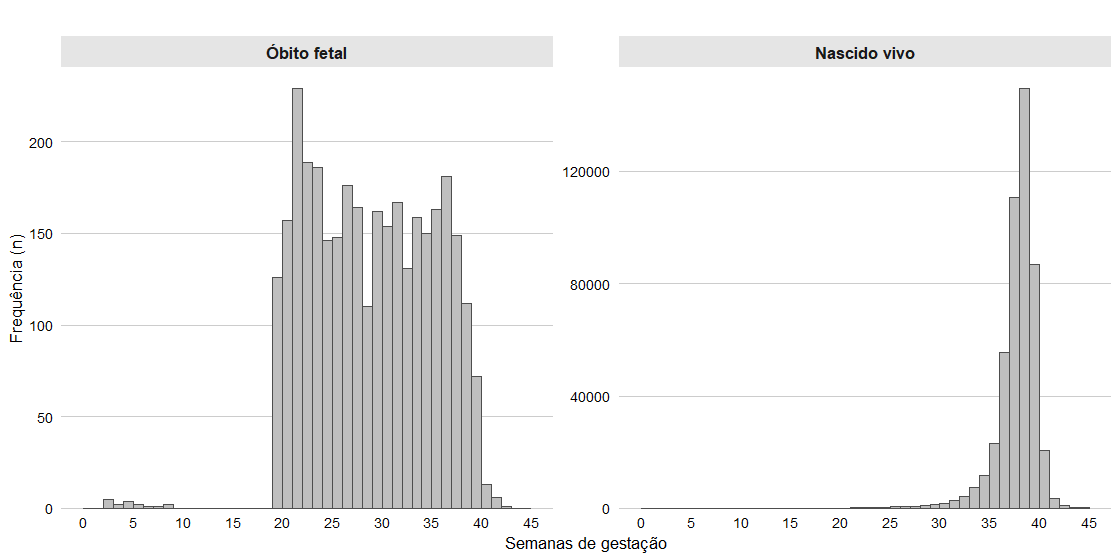
\includegraphics[width=0.9\linewidth]{figuras/histograma_ambas_causas.png}
  \fonte{Fonte: figura feita pelo autor.}
  \label{fig:histograma_ambas_causas}
\end{figure}

Nas curvas globais de Kaplan-Meier (Figura \ref{fig:0_ambos_km_global}), quando 
o óbito fetal é tratado como evento de interesse e o nascimento vivo como censura, 
a função de sobrevivência fica muito próxima de 1 durante toda a gestação, o que 
reforça a raridade desse desfecho. Quando o nascimento vivo é tratado como evento 
e os óbitos fetais como censura, observa-se uma queda acentuada da função de 
sobrevivência a partir do final do terceiro trimestre, mostrando a forte concentração 
dos desfechos em torno do termo.

%---------------------- KM globais
\begin{figure}[H]
  \centering
  \caption{Curvas de Kaplan-Meier da idade gestacional para cada desfecho}
  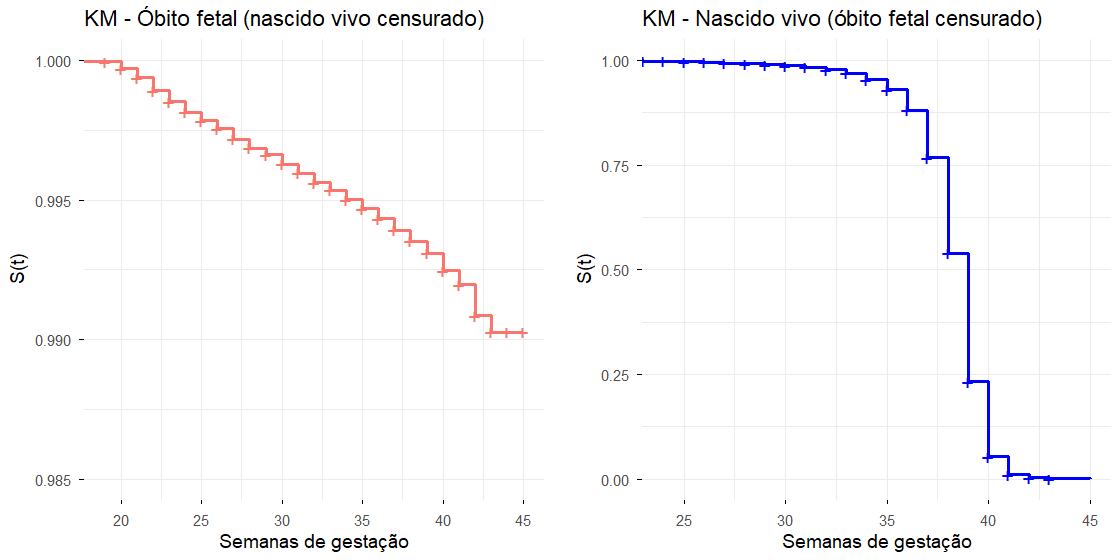
\includegraphics[width=0.9\linewidth]{figuras/0_ambos_km_global.png}
  \fonte{Fonte: figura feita pelo autor.}
  \label{fig:0_ambos_km_global}
\end{figure}

De forma complementar, as funções de incidência acumulada (CIF) por 
causa (Figura \ref{fig:cif_global_painel}) mostram a probabilidade acumulada de 
ocorrência de cada desfecho ao longo da gestação na presença de riscos 
competitivos. Para o óbito fetal, essa incidência permanece baixa em praticamente 
todo o acompanhamento. Em torno de 30 semanas, a probabilidade acumulada de óbito 
fetal foi de aproximadamente 0,37\% (CIF $\approx$ 0,0037) e, mesmo na semana 40, 
manteve-se em torno de 0,66\% (CIF $\approx$ 0,0066), o que corresponde a cerca 
de 7 óbitos fetais por 1.000 gestações.

Já a CIF para nascimento vivo cresce de forma gradual a partir do terceiro trimestre, 
atingindo aproximadamente 1,2\% em 30 semanas (CIF $\approx$ 0,0123) e cerca 
de 94\% na semana 40 (CIF $\approx$ 0,94). Entre 40 e 45 semanas, essa CIF continua 
a crescer até se aproximar de 99\%, indicando que, ao final do acompanhamento, quase 
todas as gestações terminaram em nascimento vivo, enquanto uma pequena fração evoluiu 
para óbito fetal.

%---------------------- CIF globais
\begin{figure}[H]
  \centering
  \caption{Gráficos de incidência acumulada da idade gestacional para cada desfecho.}
  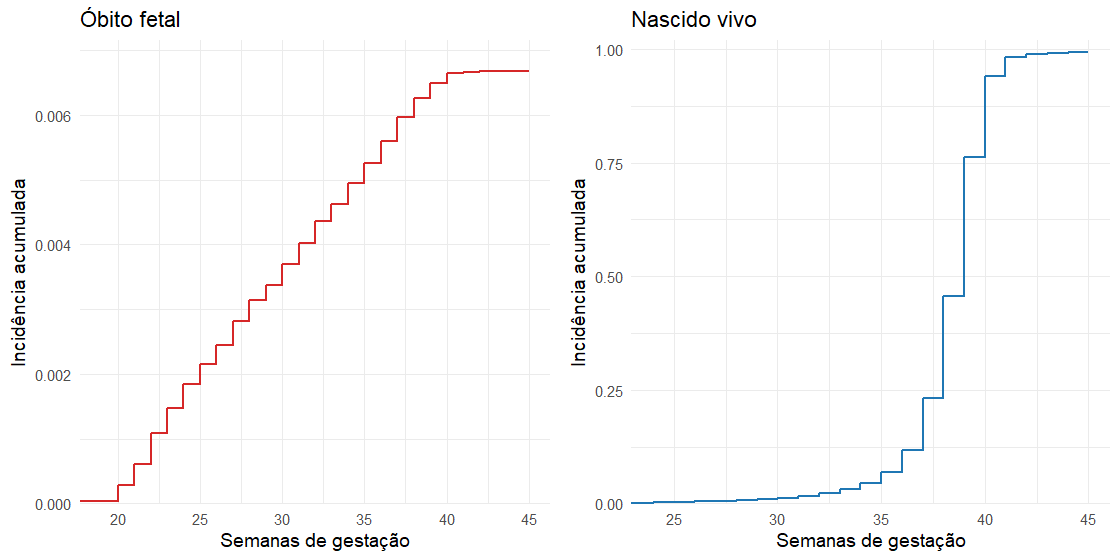
\includegraphics[width=0.9\linewidth]{figuras/cif_global_painel.png}
  \fonte{Fonte: figura feita pelo autor.}
  \label{fig:cif_global_painel}
\end{figure}

\section{Variáveis comuns para as duas causas}

Os resultados descritivos da Tabela \ref{tab:tabela-descritiva-conjunta} já apontam
diferenças entre os grupos de óbito fetal e nascido vivo e indicam heterogeneidade
inicial para a análise de sobrevivência com riscos competitivos. Como o tamanho
amostral é grande, os testes de Log-rank e de Gray tendem a detectar até diferenças
pequenas. Por isso, estatísticas $\chi^2$ muito elevadas e valores-p muito pequenos
devem ser lidos em conjunto com os gráficos e com a magnitude das diferenças
observadas.

\newpage
\begin{table}[H]
\centering
\renewcommand{\arraystretch}{1.1}
\caption{Medidas descritivas e testes de Log-rank (LR) e de Gray (GR).}
\begin{tabular}{lll}
\specialrule{0.16em}{0pt}{0pt}
\textbf{Variáveis numéricas} &
  \begin{tabular}{@{}l@{}}%
  \textbf{Óbito fetal}\\
  Média $\pm$ DP
  \end{tabular} &
  \begin{tabular}{@{}l@{}}
  \textbf{Nascido vivo}\\
  Média $\pm$ DP
  \end{tabular} \\
\specialrule{0.16em}{0pt}{0pt}
Idade materna (idademae)               & 28,92 $\pm$ 7,15 & 28,64 $\pm$ 6,59 \\
Peso ao nascer (peso)                 & 1\,381,68 $\pm$ 996,53 & 3\,132,56 $\pm$ 553,44 \\
Nº de filhos mortos previamente (qtdfilmort)    & 0,56 $\pm$ 0,83 & 0,28 $\pm$ 0,62 \\
Nº de filhos vivos previamente (qtdfilvivo)     & 1,03 $\pm$ 1,37 & 0,93 $\pm$ 1,13 \\
Idade gestacional ao parto (semagestac) & 29,39 $\pm$ 6,19 & 38,26 $\pm$ 2,13 \\
\specialrule{0.16em}{0pt}{0pt}

\textbf{Variáveis categóricas} &
  \begin{tabular}{@{}l@{}}%
    \textbf{Óbito fetal}\\[-3pt]
    {\scriptsize L: $\chi^2$ $(\text{valor-}p)$}\\[-4pt]
    {\scriptsize G: $\chi^2$ $(\text{valor-}p)$}\\[-3pt]
    n (\%)
  \end{tabular} &
  \begin{tabular}{@{}l@{}}%
    \textbf{Nascido vivo}\\[-3pt]
    {\scriptsize L: $\chi^2$ $(\text{valor-}p)$}\\[-4pt]
    {\scriptsize G: $\chi^2$ $(\text{valor-}p)$}\\[-3pt]
    n (\%)
  \end{tabular} \\

\specialrule{0.16em}{0pt}{0pt}

\begin{tabular}{@{}l@{}}Idade materna (idademae)\\< 20 anos\\20--34 anos\\$\geq 35$ anos\end{tabular} &
\begin{tabular}{@{}l@{}}
{\scriptsize L: 47{,}01 (***)};
{\scriptsize G: 40{,}36 (***)}\\
315 (9,6\,\%)\\2\,134 (65,3\,\%)\\817 (25,0\,\%)\end{tabular} &
\begin{tabular}{@{}l@{}}
{\scriptsize L: 5{\,}756 (***)};
{\scriptsize G: 4\,500\,143 (***)}\\
39\,814 (8,2\,\%)\\342\,235 (70,4\,\%)\\103\,873 (21,4\,\%)\end{tabular} \\
\hline

\begin{tabular}{@{}l@{}}Escolaridade materna (escmae2010)\\Baixa\\Média\\Alta\end{tabular} &
\begin{tabular}{@{}l@{}}
{\scriptsize L: 342 (***)};
{\scriptsize G: 344 (***)}\\
688 (21,1\,\%)\\1\,905 (58,3\,\%)\\673 (20,6\,\%)\end{tabular} &
\begin{tabular}{@{}l@{}}
{\scriptsize L: 2{\,}159 (***)};
{\scriptsize G: 1{\,}702{\,}884 (***)}\\
55\,882 (11,5\,\%)\\286\,794 (59,0\,\%)\\143\,246 (29,5\,\%)\end{tabular} \\
\hline

\begin{tabular}{@{}l@{}}Filhos vivos previamente (qtdfilvivo)\\Não\\Sim\end{tabular} &
\begin{tabular}{@{}l@{}}
{\scriptsize L: 1{,}56 (0,212)};
{\scriptsize G: 2{,}09 (0,148)}\\
1\,497 (45,8\,\%)\\1\,769 (54,2\,\%)\end{tabular} &
\begin{tabular}{@{}l@{}}
{\scriptsize L: 1{\,}113 (***)};
{\scriptsize G: 443{\,}511 (***)}\\
216\,635 (44,6\,\%)\\269\,287 (55,4\,\%)\end{tabular} \\
\hline

\begin{tabular}{@{}l@{}}Filhos mortos previamente (qtdfilmort)\\Não\\Sim\end{tabular} &
\begin{tabular}{@{}l@{}}
{\scriptsize L: 765 (***)};
{\scriptsize G: 736 (***)}\\
1\,929 (59,1\,\%)\\1\,337 (40,9\,\%)\end{tabular} &
\begin{tabular}{@{}l@{}}
{\scriptsize L: 1{\,}269 (***)};
{\scriptsize G: 3{\,}306{\,}460 (***)}\\
382\,064 (78,6\,\%)\\103\,858 (21,4\,\%)\end{tabular} \\
\hline

\begin{tabular}{@{}l@{}}Tipo de gestação (gravidez)\\Única\\Múltipla\end{tabular} &
\begin{tabular}{@{}l@{}}
{\scriptsize L: 460 (***)};
{\scriptsize G: 301 (***)}\\
3\,019 (92,4\,\%)\\247 (7,6\,\%)\end{tabular} &
\begin{tabular}{@{}l@{}}
{\scriptsize L: 49{\,}927 (***)};
{\scriptsize G: -2{\,}361 (0{,}99)}\\
473\,046 (97,4\,\%)\\12\,876 (2,6\,\%)\end{tabular} \\
\hline

\begin{tabular}{@{}l@{}}Tipo de parto (parto)\\Vaginal\\Cesáreo\end{tabular} &
\begin{tabular}{@{}l@{}}
{\scriptsize L: 1{\,}334 (***)};
{\scriptsize G: 1{\,}376 (***)}\\
2\,310 (70,7\,\%)\\956 (29,3\,\%)\end{tabular} &
\begin{tabular}{@{}l@{}}
{\scriptsize L: 4{\,}115 (***)};
{\scriptsize G: 314{\,}658 (***)}\\
189\,360 (39,0\,\%)\\296\,562 (61,0\,\%)\end{tabular} \\
\hline

\begin{tabular}{@{}l@{}}Faixa de peso ao nascer (peso)\\< 2\,500 g\\2\,500--3\,999 g\\$\geq 4\,000$ g\end{tabular} &
\begin{tabular}{@{}l@{}}
{\scriptsize L: 24{\,}947 (***)};
{\scriptsize G: 18{\,}759 (***)}\\
2\,720 (83,3\,\%)\\511 (15,6\,\%)\\35 (1,1\,\%)\end{tabular} &
\begin{tabular}{@{}l@{}}
{\scriptsize L: 136{\,}887 (***)};
{\scriptsize G: 5{\,}204{\,}921 (***)}\\
48\,219 (9,9\,\%)\\420\,310 (86,5\,\%)\\17\,393 (3,6\,\%)\end{tabular} \\
\hline

\begin{tabular}{@{}l@{}}Local de ocorrência do parto (lococornasc)\\Hospital\\Outros\end{tabular} &
\begin{tabular}{@{}l@{}}
{\scriptsize L: 287 (***)};
{\scriptsize G: 288 (***)}\\
3\,183 (97,5\,\%)\\83 (2,5\,\%)\end{tabular} &
\begin{tabular}{@{}l@{}}
{\scriptsize L: 39{,}5 (***)};
{\scriptsize G: 71{\,}669{\,}914 (***)}\\
483\,632 (99,5\,\%)\\2\,290 (0,5\,\%)\end{tabular} \\
\hline

\begin{tabular}{@{}l@{}}Sexo do recém-nascido (sexo)\\Masculino\\Feminino\end{tabular} &
\begin{tabular}{@{}l@{}}
{\scriptsize L: 6{,}77 (**)}; 
{\scriptsize G: 6{,}14 (0,013)}\\
1\,738 (53,2\,\%)\\1\,528 (46,8\,\%)\end{tabular} &
\begin{tabular}{@{}l@{}}
{\scriptsize L: 110 (***)};
{\scriptsize G: 750{\,}287 (***)}\\
248\,019 (51,0\,\%)\\237\,903 (49,0\,\%)\end{tabular} \\
\hline

\end{tabular}
\fonte{n (\%): frequências em relação ao total de indivíduos de cada grupo,
considerando registros com informação válida de idade gestacional e da variável.
L e G: testes de Log-rank e de Gray, com estatística do teste ($\chi^2$) e
valor-p. Significância: *** $p<0{,}001$; ** $p<0{,}01$. Fonte: elaboração do
autor.}
\label{tab:tabela-descritiva-conjunta} 
\end{table}

Nas variáveis numéricas, o grupo de óbito fetal apresentou, em média, peso ao
nascer bem menor que o grupo de nascidos vivos (1.381,68 $\pm$ 996,53 e
3.132,56 $\pm$ 553,44, respectivamente), além de idade gestacional ao parto muito
menor (29,39 $\pm$ 6,19 e 38,26 $\pm$ 2,13, respectivamente). Assim, é possível notar que 
os óbitos fetais se concentraram em gestações mais precoces e com pesos menores
no momento do desfecho. Além disso, o número médio de filhos mortos previamente
foi maior nesse grupo (0,56 $\pm$ 0,83 contra 0,28 $\pm$ 0,62 em nascidos vivos),
o que sugere histórico reprodutivo menos favorável em parte dessas gestantes.

Entre as variáveis categóricas, a idade materna chama atenção. O grupo com menos de 20 anos correspondeu a
9,6\% dos óbitos fetais e 8,2\% dos nascidos vivos, no grupo de 20--34 anos esses valores foram de 65,3\% para óbitos fetais e 70,4\% para nascidos vivos, enquanto o grupo com 35 anos 
ou mais correspondeu a 25,0\% e 21,4\%, respectivamente. Nos gráficos de Kaplan-Meier da Figura \ref{fig:kmglobal_idade_mae}, as curvas
por idade materna sugerem diferenças no tempo até o desfecho. Para óbito fetal, o
teste de Log-rank foi significativo ($\chi^2=47{,}01$; $p<0{,}001$). Nos óbitos
fetais, as medianas (Q1--Q3) foram de 28 semanas (24--33) nas gestantes com menos
de 20 anos, 29 semanas (24--35) entre 20 e 34 anos e 30 semanas (24--35) no grupo com 35 anos ou
mais. Para nascimento vivo, o Log-rank também foi significativo
($\chi^2=5\,756$; $p<0{,}001$), com medianas de 39 semanas (38--40), 39 semanas (38--39) e 38 semanas (37--39), respectivamente. 

%---------------------------------------------------------
%---------------------- idademae
%---------------------------------------------------------

%---------------------- KM
\begin{figure}[H]
  \centering
  \caption{Gráficos de Kaplan-Meier da variável idademae para cada desfecho.}
  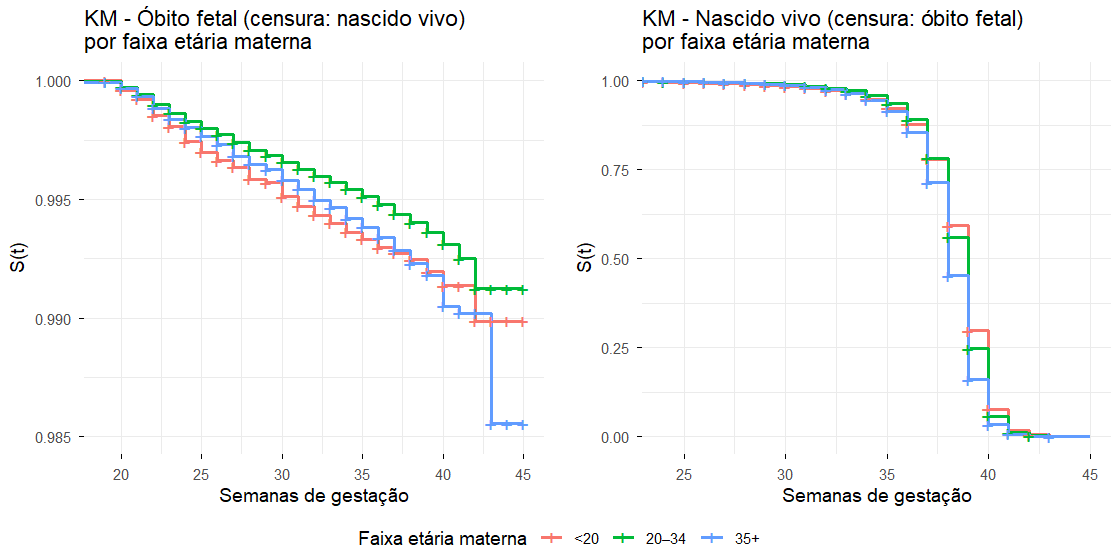
\includegraphics[width=0.9\linewidth]{figuras/kmglobal_idade_mae.png}
  \fonte{Fonte: figura feita pelo autor.}
  \label{fig:kmglobal_idade_mae}
\end{figure}
%---------------------- CIF
Na Figura \ref{fig:cif_idademae_painel_ambos}, sob a perspectiva de óbito fetal, o grupo
com menos de 20 anos apresentou a maior CIF durante grande parte do
acompanhamento: 0,49\% na semana 30, 0,66\% na semana 35 e 0,78\% na semana 40.
No grupo com 35 anos ou mais, os valores foram muito próximos ao final do
seguimento, passando de 0,42\% para 0,61\% e 0,78\%, enquanto o grupo de 20 a 34
anos manteve os menores valores, com 0,34\%, 0,48\% e 0,61\%, respectivamente.
O teste de Gray confirmou evidência de diferença para óbito fetal
($\chi^2=40{,}36$; $p<0{,}001$). Para nascimento vivo, o padrão foi diferente:
na semana 30 a maior CIF apareceu entre as menores de 20 anos (1,66\%), mas a
partir da semana 35 o grupo com 35 anos ou mais passou a concentrar mais
nascimentos vivos, com 8,51\% na semana 35 e 95,92\% na semana 40, contra 7,75\%
e 91,50\% nas menores de 20 anos e 6,46\% e 93,71\% no grupo de 20 a 34 anos. O
teste de Gray também apontou diferença para nascimento vivo
($\chi^2=4\,500\,143$; $p<0{,}001$).
\begin{figure}[H]
  \centering
  \caption{Gráficos de incidência acumulada da variável idademae para cada desfecho.}
  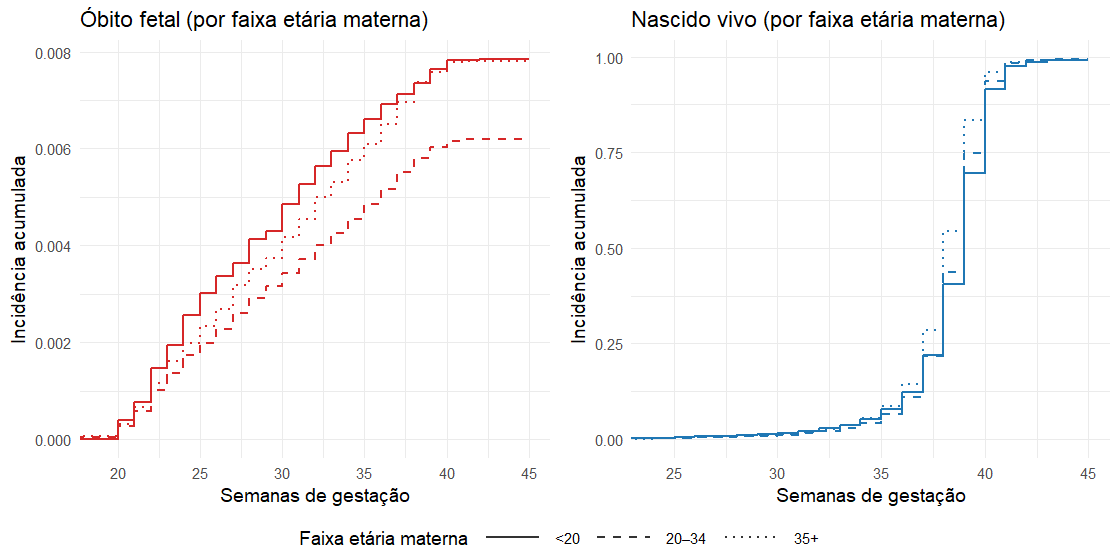
\includegraphics[width=0.9\linewidth]{figuras/cif_idademae_painel_ambos.png}
  \fonte{Fonte: figura feita pelo autor.}
  \label{fig:cif_idademae_painel_ambos}
\end{figure}

Assim, a idade materna apresentou heterogeneidade nos dois desfechos. Na
perspectiva do óbito fetal, o grupo de 20 a 34 anos teve menor probabilidade
acumulada de óbito fetal, enquanto os extremos de idade, especialmente menores de
20 anos durante boa parte do acompanhamento e 35 anos ou mais ao final da
gestação, concentraram resultados menos favoráveis para gestação.

%---------------------------------------------------------
%---------------------- escolaridade
%---------------------------------------------------------

%---------------------- KM
Nos gráficos de Kaplan-Meier da Figura \ref{fig:kmglobal_escmae2010}, a
escolaridade materna sugere diferenças mais visíveis entre as curvas no óbito fetal do que no
nascimento vivo. O Log-rank foi significativo nas duas análises
($\chi^2=342$ para óbito fetal e $\chi^2=2\,159$ para nascimento vivo;
$p<0{,}001$ em ambos), indicando que as curvas não devem ser tratadas como
equivalentes. Nos óbitos fetais, as medianas (Q1--Q3) foram de 30 semanas
(24--35) na baixa escolaridade, 30 semanas (24--35) na escolaridade média e 28 semanas (23--34)
na alta escolaridade. Entre os nascidos vivos, as medianas foram de 39 semanas
em todos os grupos, com intervalo interquartílico de 37--40 na baixa
escolaridade, 38--40 na média e 38--39 na alta.
\begin{figure}[H]
  \centering
  \caption{Gráficos de Kaplan-Meier da variável escmae2010 referente a escolaridade materna,
  para cada desfecho.}
  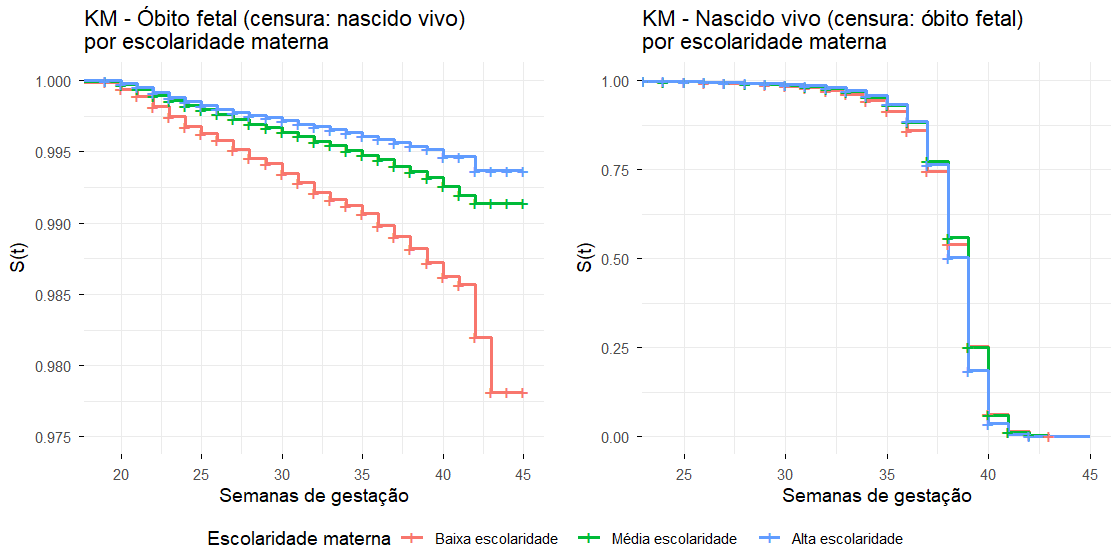
\includegraphics[width=0.9\linewidth]{figuras/kmglobal_escmae2010.png}
  \fonte{Fonte: figura feita pelo autor.}
  \label{fig:kmglobal_escmae2010}
\end{figure}
%---------------------- CIF
Na Figura \ref{fig:cif_escmae2010_painel_ambos}, na semana 40, a CIF de óbito
fetal foi de 1,21\% na baixa escolaridade, 0,66\% na escolaridade média e 0,47\%
na alta escolaridade. O Gray reforçou essa diferença no óbito fetal
($\chi^2=344$; $p<0{,}001$). Entre os nascidos vivos, as curvas também apresentaram diferenças, mas com menor contraste visual, alcançando 92,50\% na baixa
escolaridade, 93,37\% na média e 95,85\% na alta escolaridade na semana 40
($\chi^2=1\,702\,884$; $p<0{,}001$). Em conjunto, os resultados sugerem situação
mais favorável para gestação no grupo de maior escolaridade, embora parte dessa diferença
provavelmente represente condições sociais e assistenciais associadas.
\begin{figure}[H]
  \centering
  \caption{Gráficos de incidência acumulada da variável escmae2010 referente a escolaridade
  materna, para cada desfecho.}
  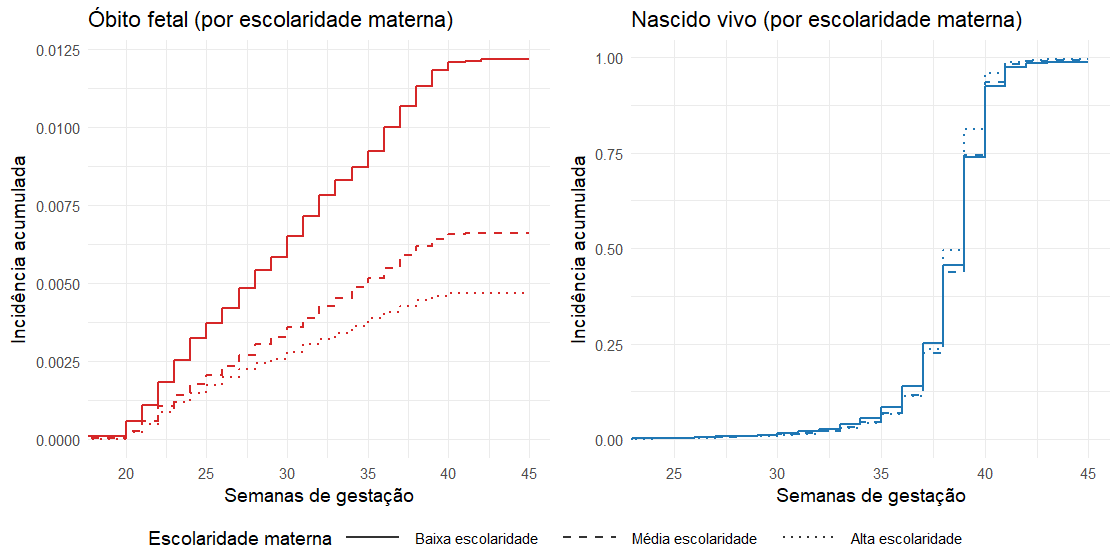
\includegraphics[width=0.9\linewidth]{figuras/cif_escmae2010_painel_ambos.png}
  \fonte{Fonte: figura feita pelo autor.}
  \label{fig:cif_escmae2010_painel_ambos}
\end{figure}

Por tanto, a escolaridade materna aponta para um detalhe importante, com menor
incidência acumulada de óbito fetal e maior concentração de nascimentos vivos no
grupo de maior escolaridade. Esse achado deve ser entendido como marcador de
condições sociais e assistenciais, e não como efeito isolado da escolaridade.

%---------------------------------------------------------
%---------------------- quantidade de filhos vivos
%---------------------------------------------------------

%---------------------- KM
Nos gráficos de Kaplan-Meier da Figura \ref{fig:kmglobal_filvivo}, a presença de
filhos vivos previamente sugere pouco contraste entre os grupos. Essa impressão é coerente com os testes para óbito fetal, que não
foram significativos (Log-rank: $\chi^2=1{,}56$, $p=0{,}212$; Gray:
$\chi^2=2{,}09$, $p=0{,}148$). Para nascimento vivo, o Log-rank foi significativo
($\chi^2=1\,113$; $p<0{,}001$), mas a diferença foi pequena na escala das
semanas. Entre os óbitos fetais, mulheres sem filhos vivos prévios tiveram
mediana de 28 semanas (23--34), enquanto aquelas com esse antecedente tiveram
mediana de 30 semanas (25--35). Entre os nascidos vivos, as medianas foram de 39
semanas nos dois grupos, com Q1--Q3 de 38--40 no grupo sem filhos vivos prévios
e 38--39 no grupo com esse antecedente.
\begin{figure}[H]
  \centering
  \caption{Gráficos de Kaplan-Meier da variável qtdfilvivo referente a quantidade de filhos
  vivos anteriores, para cada desfecho.}
  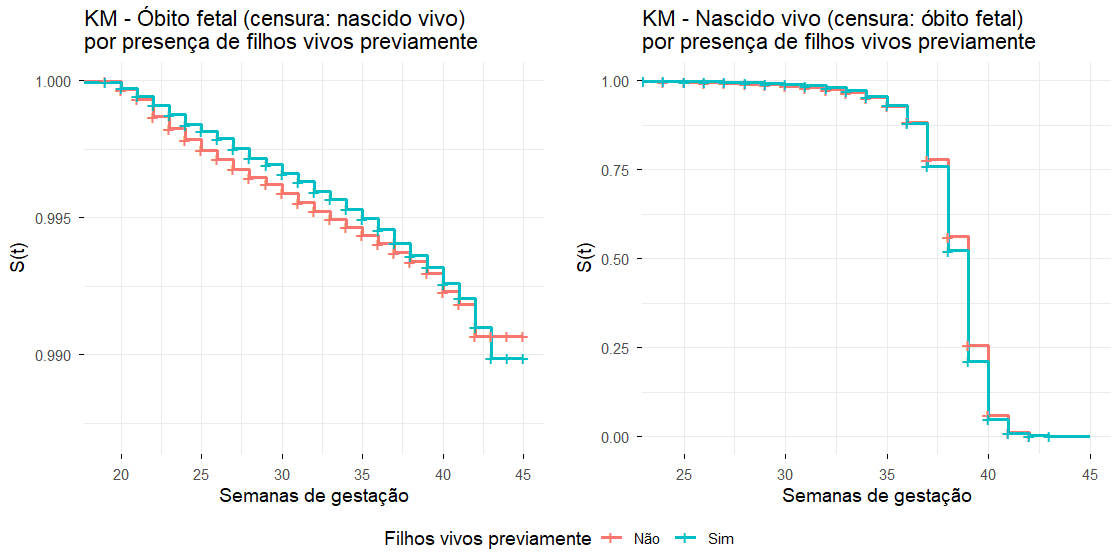
\includegraphics[width=0.9\linewidth]{figuras/kmglobal_filvivo.png}
  \fonte{Fonte: figura feita pelo autor.}
  \label{fig:kmglobal_filvivo}
\end{figure}
%---------------------- CIF
Na Figura \ref{fig:cif_filvivo_painel_ambos}, a incidência acumulada confirma
que o contraste foi pequeno no óbito fetal: na semana 40, a CIF foi de 0,68\%
entre mulheres sem filhos vivos prévios e de 0,65\% entre aquelas com esse
antecedente. Para nascimento vivo, o Gray foi significativo
($\chi^2=443\,511$; $p<0{,}001$), mas as curvas também ficaram próximas. Ao fim
do acompanhamento, o grupo com filhos vivos prévios acumulou proporção
ligeiramente maior de nascimentos até a semana 40 (94,53\% contra 93,34\%).
Portanto, trata-se de diferença estatisticamente detectável apenas na ótica dos
nascidos vivos, mas pequena do ponto de vista absoluto.
\begin{figure}[H]
  \centering
  \caption{Gráficos de incidência acumulada da variável qtdfilvivo referente a quantidade de
  filhos vivos anteriores, para cada desfecho.}
  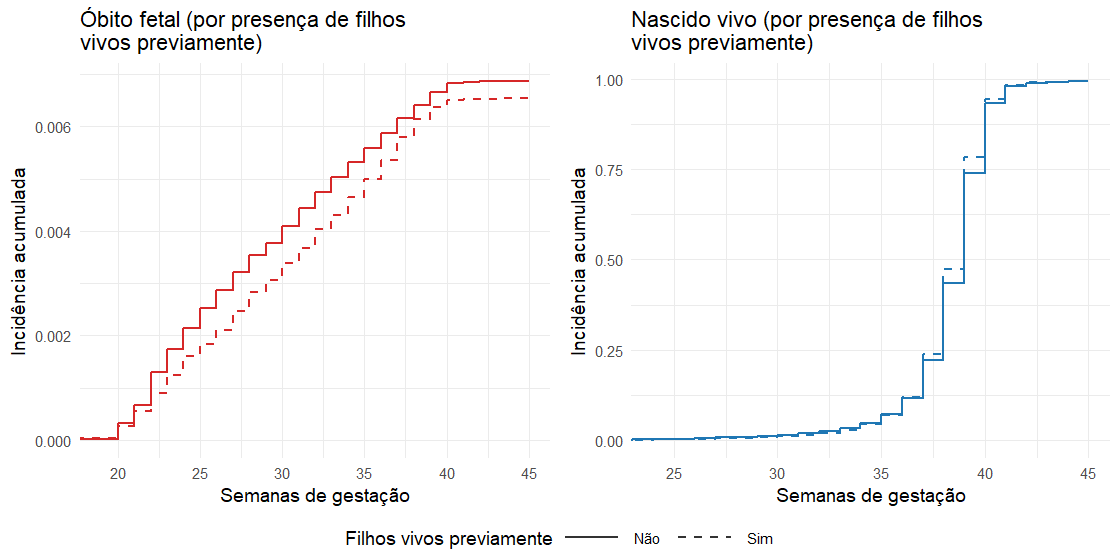
\includegraphics[width=0.9\linewidth]{figuras/cif_filvivo_painel_ambos.png}
  \fonte{Fonte: figura feita pelo autor.}
  \label{fig:cif_filvivo_painel_ambos}
\end{figure}

No geral, a presença de filhos vivos previamente não mostrou um padrão forte
para diferenciar o tempo até o desfecho. A variável parece ter pouca relevância
prática isolada, principalmente para óbito fetal, em que os testes e as curvas
ficaram próximos entre os grupos.

%---------------------------------------------------------
%---------------------- quantidade de filhos mortos
%---------------------------------------------------------

%---------------------- KM
Nos gráficos de Kaplan-Meier da Figura \ref{fig:kmglobal_filmort}, o antecedente
de filhos mortos previamente sugere diferença entre os grupos. O
Log-rank foi significativo para óbito fetal ($\chi^2=765$; $p<0{,}001$) e para
nascimento vivo ($\chi^2=1\,269$; $p<0{,}001$). Descritivamente, entre os óbitos
fetais, gestantes com esse antecedente tiveram mediana de 28 semanas (24--34),
enquanto as demais tiveram mediana de 30 semanas (24--35). Entre os nascidos
vivos, as medianas foram de 38 semanas (37--39) para mulheres com filhos mortos
prévios e de 39 semanas (38--39) para as demais.
\begin{figure}[H]
  \centering
  \caption{Gráficos de Kaplan-Meier da variável qtdfilmort referente a quantidade de filhos
  mortos anteriores, para cada desfecho.}
  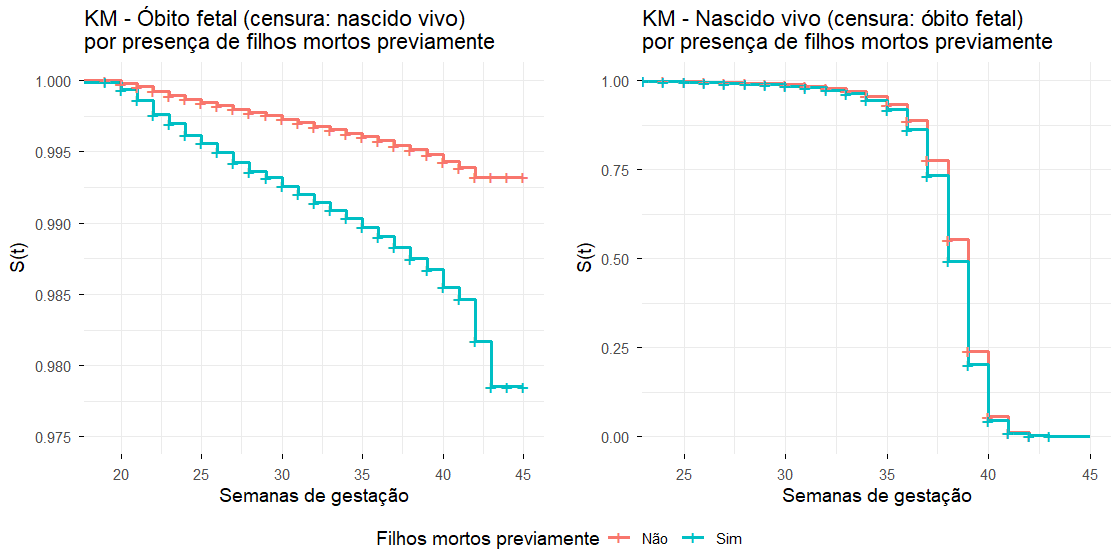
\includegraphics[width=0.9\linewidth]{figuras/kmglobal_filmort.png}
  \fonte{Fonte: figura feita pelo autor.}
  \label{fig:kmglobal_filmort}
\end{figure}
%---------------------- CIF
Na Figura \ref{fig:cif_filmort_painel_ambos}, entre os óbitos fetais, gestantes
com esse antecedente apresentaram CIF mais alta em todas as semanas avaliadas,
passando de 0,74\% na semana 30 para 1,26\% na semana 40, enquanto no grupo sem
esse antecedente os valores foram de 0,27\% e 0,50\%. O teste de Gray para óbito fetal
foi significativo ($\chi^2=736$; $p<0{,}001$). Entre os nascidos vivos, a
diferença foi menor, mas na mesma direção, com CIF de 94,25\% na semana 40 entre
mulheres com filhos mortos prévios e de 93,93\% entre as demais
($\chi^2=3\,306\,460$; $p<0{,}001$). Embora há evidência de diferença entre os grupos, no caso de nascidos vivos os resultados são similares em magnitude.
\begin{figure}[H]
  \centering
  \caption{Gráficos de incidência acumulada da variável qtdfilmort referente a quantidade de
  filhos mortos anteriores, para cada desfecho.}
  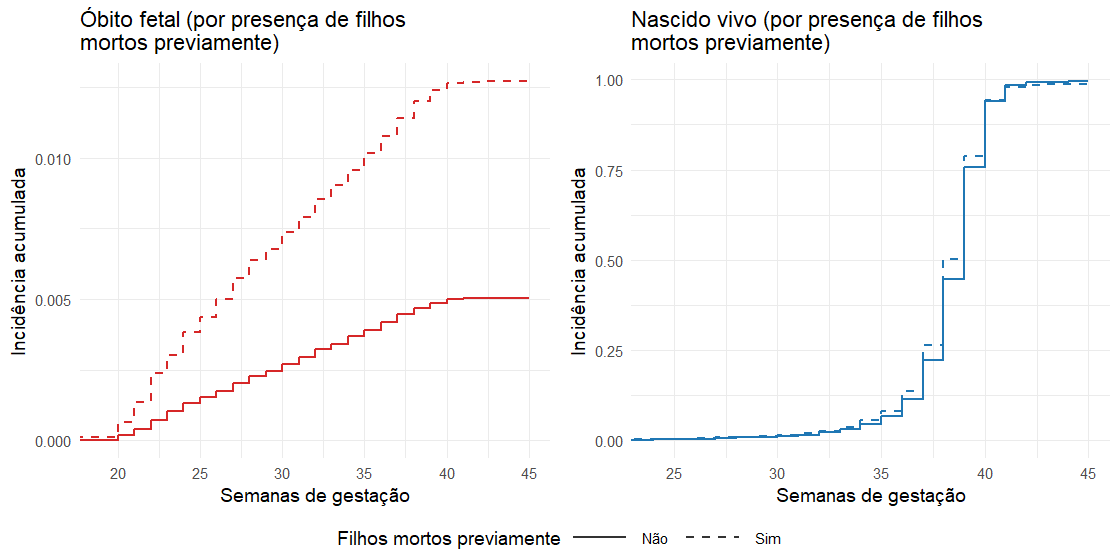
\includegraphics[width=0.9\linewidth]{figuras/cif_filmort_painel_ambos.png}
  \fonte{Fonte: figura feita pelo autor.}
  \label{fig:cif_filmort_painel_ambos}
\end{figure}

Em conjunto, o antecedente de filhos mortos previamente indica um perfil
reprodutivo menos favorável para gestação, sobretudo na ótica de óbito fetal. A maior CIF de óbito
fetal nesse grupo sugere maior vulnerabilidade obstétrica, enquanto nos nascidos
vivos a diferença existiu, mas foi menor em magnitude.

%---------------------------------------------------------
%---------------------- tipo de gravidez
%---------------------------------------------------------

%---------------------- KM
Nos gráficos de Kaplan-Meier da Figura \ref{fig:kmglobal_gravidez}, o tipo de
gestação sugere uma das separações mais claras da análise. De forma descritiva, as
gestações múltiplas terminaram mais cedo que as gestações únicas nas duas
perspectivas. Entre os óbitos fetais, as gestações múltiplas tiveram mediana de
26 semanas (22--32), contra 30 semanas (24--35) nas gestações únicas. Entre os
nascidos vivos, as medianas foram de 36 semanas (34--37) nas múltiplas e 39
semanas (38--39) nas únicas. O Log-rank confirmou forte evidência de diferença entre as curvas 
para óbito fetal ($\chi^2=460$; $p<0{,}001$) e para nascimento vivo
($\chi^2=49\,927$; $p<0{,}001$).
\begin{figure}[H]
  \centering
  \caption{Gráficos de Kaplan-Meier da variável gravidez referente ao tipo de gravidez, para
  cada desfecho.}
  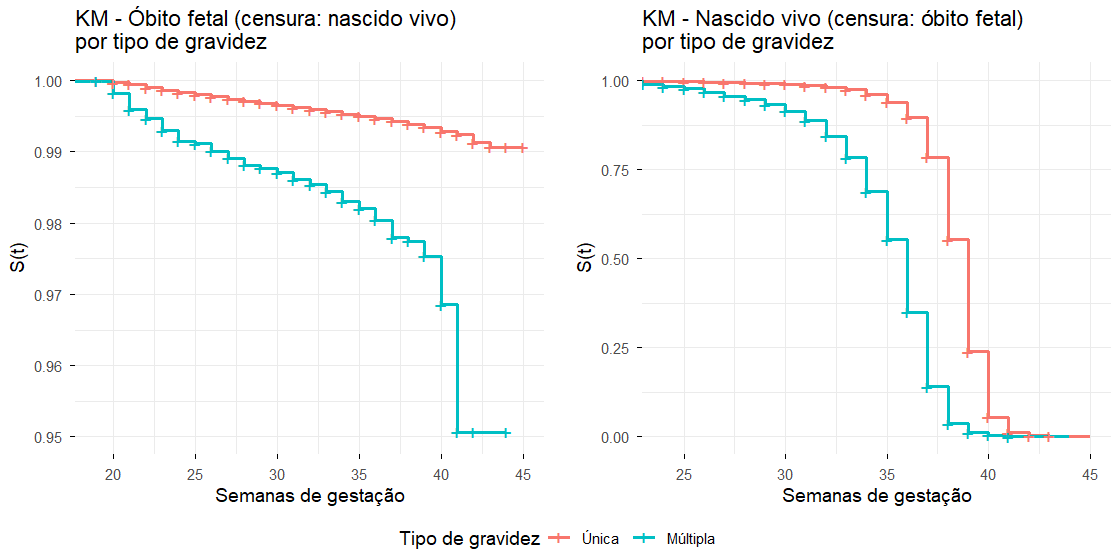
\includegraphics[width=0.9\linewidth]{figuras/kmglobal_gravidez.png}
  \fonte{Fonte: figura feita pelo autor.}
  \label{fig:kmglobal_gravidez}
\end{figure}
%---------------------- CIF
Na Figura \ref{fig:cif_gravidez_painel_ambos}, a CIF permite dimensionar melhor
essa diferença no tempo gestacional. Na ótica do óbito fetal, a incidência
acumulada das gestações múltiplas foi de 1,27\% na semana 30, 1,68\% na semana
35 e 1,87\% na semana 40, enquanto nas gestações únicas os valores foram de
0,34\%, 0,49\% e 0,63\%. O teste de Gray para óbito fetal também apontou diferença 
significativa ($\chi^2=301$; $p<0{,}001$). Para nascimento vivo, a separação foi ainda mais
evidente: nas gestações múltiplas, a CIF já era de 8,51\% na semana 30, chegou a
43,95\% na semana 35 e a 97,71\% na semana 40, contra 1,03\%, 5,99\% e 93,90\%
nas gestações únicas. Assim, esses resultados refletem a maior frequência de
partos pré-termo em gestações múltiplas.
\begin{figure}[H]
  \centering
  \caption{Gráficos de incidência acumulada da variável gravidez referente ao tipo de
  gravidez, para cada desfecho.}
  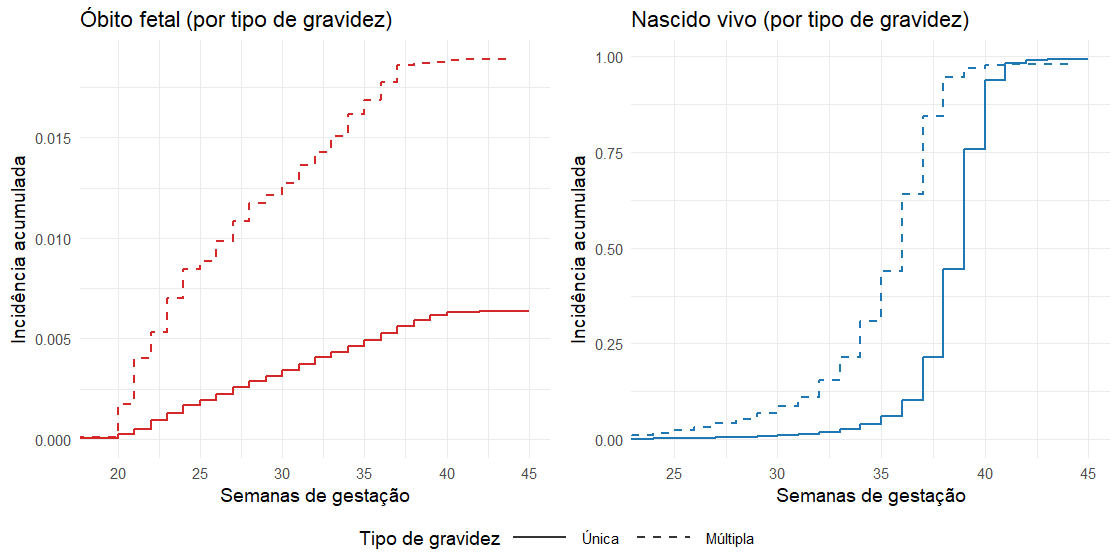
\includegraphics[width=0.9\linewidth]{figuras/cif_gravidez_painel_ambos.png}
  \fonte{Fonte: figura feita pelo autor.}
  \label{fig:cif_gravidez_painel_ambos}
\end{figure}

Portanto, o tipo de gestação foi uma das variáveis com conclusão mais clara:
gestações múltiplas se associaram a desfechos em idades gestacionais mais
precoces e a maior probabilidade acumulada de eventos antes do termo,
principalmente no ambito dos nascidos vivos.

%---------------------------------------------------------
%---------------------- tipo de parto
%---------------------------------------------------------

%---------------------- KM
Nos gráficos de Kaplan-Meier da Figura \ref{fig:kmglobal_parto}, o tipo de parto
sugere distribuições distintas do tempo até o desfecho. O Log-rank foi
significativo para óbito fetal ($\chi^2=1\,334$; $p<0{,}001$) e para nascimento
vivo ($\chi^2=4\,115$; $p<0{,}001$). Nos óbitos fetais, partos vaginais tiveram
mediana de 27 semanas (23--32), enquanto os cesáreos tiveram mediana de 34
semanas (30--37). Entre os nascidos vivos, a mediana foi de 39 semanas nos dois
grupos, mas o intervalo interquartílico foi de 37--39 nos cesáreos e de 38--40
nos vaginais. Como complemento, as médias $\pm$ DP (mediana) foram de 38,15
$\pm$ 2,07 (39) nos cesáreos e 38,41 $\pm$ 2,21 (39) nos vaginais, sugerindo
deslocamento discreto para idades gestacionais um pouco menores no grupo
cesáreo.
\begin{figure}[H]
  \centering
  \caption{Gráficos de Kaplan-Meier da variável parto referente ao tipo de parto, para cada
  desfecho.}
  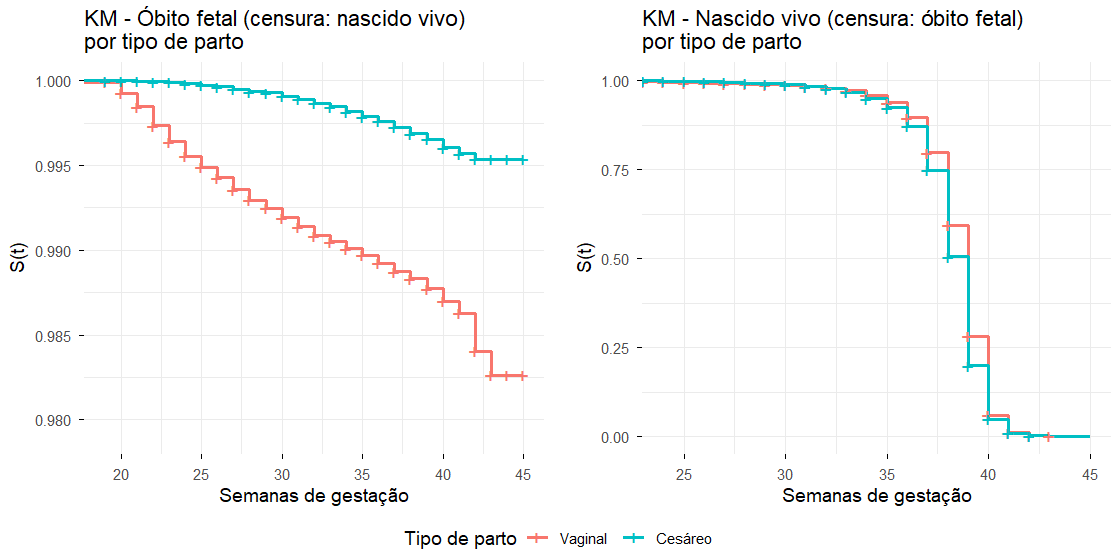
\includegraphics[width=0.9\linewidth]{figuras/kmglobal_parto.png}
  \fonte{Fonte: figura feita pelo autor.}
  \label{fig:kmglobal_parto}
\end{figure}
%---------------------- CIF
Na Figura \ref{fig:cif_parto_painel_ambos}, entre os óbitos fetais, os casos
classificados como parto vaginal se concentraram em idades
gestacionais mais precoces, com CIF de 0,80\% na semana 30 e 1,20\% na semana 40,
contra 0,09\% e 0,32\% entre os partos cesáreos. O teste de Gray para óbito fetal foi
significativo ($\chi^2=1\,376$; $p<0{,}001$). Entre os nascidos vivos, os partos
cesáreos apresentaram incidência acumulada um pouco maior em idades
gestacionais anteriores ou próximas do termo, com CIF de 7,57\% na semana 35 e
94,73\% na semana 40, contra 6,13\% e 92,87\% nos partos vaginais
($\chi^2=314\,658$; $p<0{,}001$). Como o tipo de parto é definido no momento do
desfecho, essa variável deve ser interpretada como parte do processo assistencial
do parto, e não como causa isolada do tempo até o parto.
\begin{figure}[H]
  \centering
  \caption{Gráficos de incidência acumulada da variável parto referente ao tipo de parto,
  para cada desfecho.}
  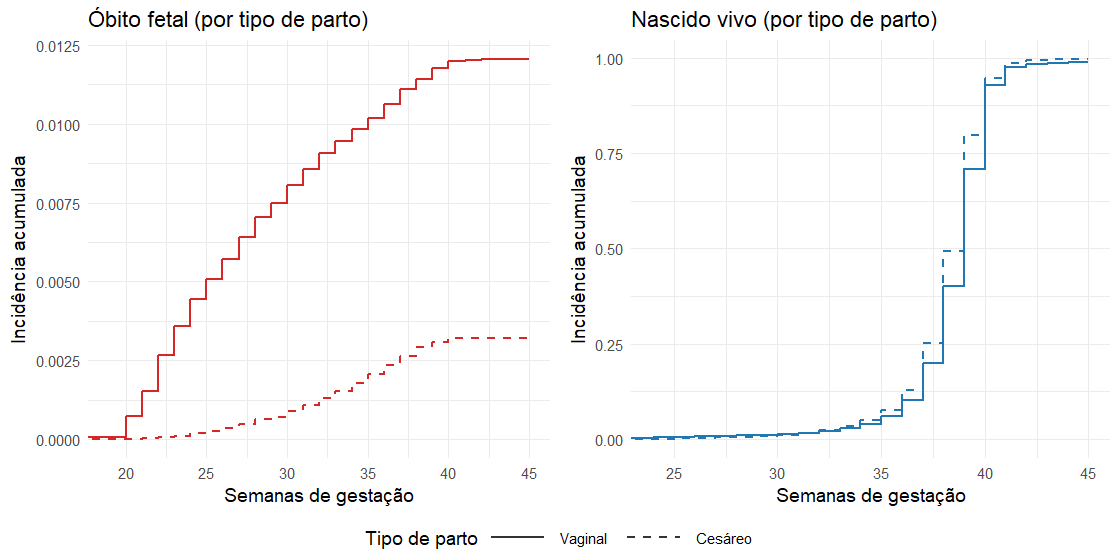
\includegraphics[width=0.9\linewidth]{figuras/cif_parto_painel_ambos.png}
  \fonte{Fonte: figura feita pelo autor.}
  \label{fig:cif_parto_painel_ambos}
\end{figure}

De forma geral, o tipo de parto apresenta diferenças no tempo gestacional, mas sua
interpretação deve permanecer vinculada ao contexto assistencial do parto. Os resultados
mostram associação com o momento do desfecho, principalmente pela concentração de
óbitos fetais mais precoces em partos vaginais e de nascimentos vivos
ligeiramente mais precoces em cesáreas.

%---------------------------------------------------------
%---------------------- peso
%---------------------------------------------------------

%---------------------- KM 
Nos gráficos de Kaplan-Meier da Figura \ref{fig:kmglobal_peso_categorico}, a
faixa de peso ao nascer apresenta o contraste mais evidente entre as variáveis em comuns das bases de dados. O Log-rank foi significativo para óbito fetal ($\chi^2=24\,947$;
$p<0{,}001$) e para nascimento vivo ($\chi^2=136\,887$; $p<0{,}001$). Entre os
óbitos fetais, o grupo com menos de 2.500 g teve mediana de 27 semanas (23--32),
enquanto as faixas de 2.500 a 3.999 g e de 4.000 g ou mais tiveram mediana de 37
semanas, com Q1--Q3 de 36--39 e 36,5--38, respectivamente. Entre os nascidos
vivos, o baixo peso apresentou mediana de 36 semanas (33--37), enquanto as faixas
de 2.500 a 3.999 g e de 4.000 g ou mais tiveram mediana de 39 semanas, com
Q1--Q3 de 38--39 e 39--40.
\begin{figure}[H]
  \centering
  \caption{Gráficos de Kaplan-Meier da variável peso, para cada desfecho.}
  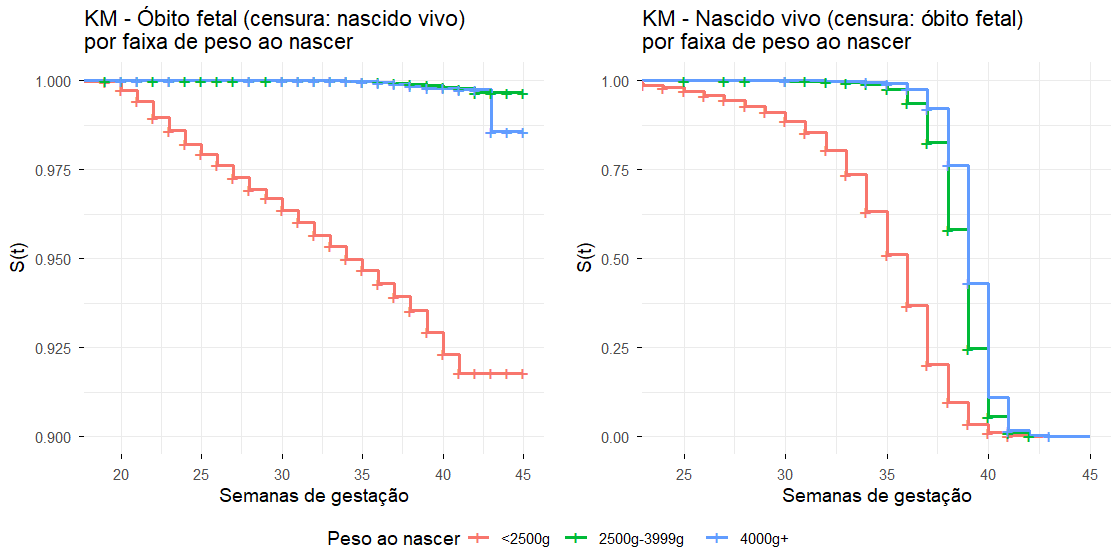
\includegraphics[width=0.9\linewidth]{figuras/kmglobal_peso_categorico.png}
  \fonte{Fonte: figura feita pelo autor.}
  \label{fig:kmglobal_peso_categorico}
\end{figure}
%---------------------- CIF 
Na Figura \ref{fig:cif_peso_categorico_painel_ambos}, entre os óbitos fetais com
peso inferior a 2.500 g, a CIF chegou a 3,52\% na semana 30 e a
5,33\% na semana 40, enquanto nas faixas de 2.500 a 3.999 g e de 4.000 g ou mais
os valores ficaram próximos de zero até o fim do acompanhamento
($\chi^2=18\,759$; $p<0{,}001$ no teste de Gray). Entre os nascidos vivos, o
grupo com menos de 2.500 g também concentrou os desfechos mais precoces,
alcançando CIF de 11,04\% na semana 30 e 46,85\% na semana 35, contra 0,10\% e
2,44\% na faixa de 2.500 a 3.999 g e 0,03\% e 0,85\% na faixa de 4.000 g ou mais
($\chi^2=5\,204\,921$; $p<0{,}001$). Como o peso é observado no momento do
desfecho, essa relação deve ser lida como associação com a idade gestacional, e
não como causa do parto ou do óbito fetal.
\begin{figure}[H]
  \centering
  \caption{Gráficos de incidência acumulada da variável peso, para cada desfecho.}
  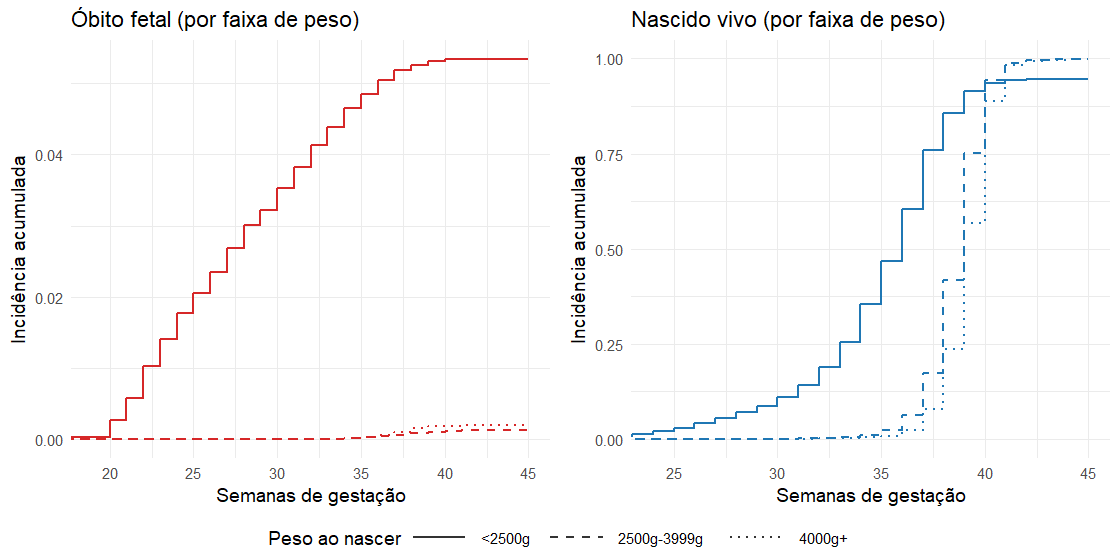
\includegraphics[width=0.9\linewidth]{figuras/cif_peso_categorico_painel_ambos.png}
  \fonte{Fonte: figura feita pelo autor.}
  \label{fig:cif_peso_categorico_painel_ambos}
\end{figure}

Assim, o baixo peso ao nascer foi um dos marcadores mais fortes de
desfechos em idades gestacionais precoces. A interpretação principal é que peso e
idade gestacional estão fortemente relacionados no momento do desfecho, de modo
que essa variável descreve um perfil clínico mais vulnerável, sem indicar
causalidade direta.

%---------------------------------------------------------
%---------------------- local de ocorrência
%---------------------------------------------------------

%---------------------- KM 
Nos gráficos de Kaplan-Meier da Figura \ref{fig:kmglobal_lococornasc}, o local de
ocorrência do parto sugere diferença entre as curvas, mas a interpretação exige
cautela devido ao número muito pequeno de registros fora do hospital. O Log-rank
foi significativo para óbito fetal ($\chi^2=287$; $p<0{,}001$) e para nascimento
vivo ($\chi^2=39{,}5$; $p<0{,}001$). Ainda assim, as medianas observadas foram
iguais entre hospital e outros locais em cada desfecho: 29 semanas para ambos nos óbitos
fetais e 39 semanas nos nascidos vivos. Os intervalos interquartílicos também
foram próximos, de 24--35 e 25--35 nos óbitos fetais, e de 38--39 e 38--40 nos
nascidos vivos, respectivamente.
\begin{figure}[H]
  \centering
  \caption{Gráficos de Kaplan-Meier da variável lococornasc referente ao local de
  ocorrência, para cada desfecho.}
  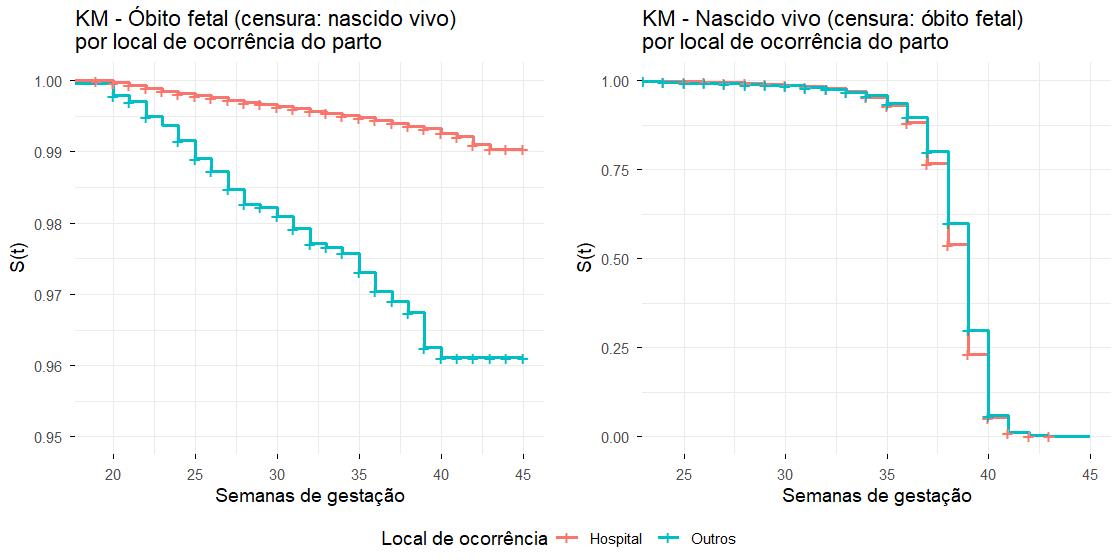
\includegraphics[width=0.9\linewidth]{figuras/kmglobal_lococornasc.png}
  \fonte{Fonte: figura feita pelo autor.}
  \label{fig:kmglobal_lococornasc}
\end{figure}
%---------------------- CIF 
Na Figura \ref{fig:cif_lococornasc_painel_ambos}, a interpretação continua
exigindo cautela porque a categoria ``Outros'' foi muito pequena, com 83 óbitos
fetais e 2.290 nascidos vivos. Mesmo assim, no óbito fetal a CIF foi mais alta
fora do ambiente
hospitalar, chegando a 1,90\% na semana 30 e 3,50\% na semana 40, contra 0,36\%
e 0,65\% nos partos hospitalares ($\chi^2=288$; $p<0{,}001$ no teste de Gray).
Entre os nascidos vivos, a diferença foi menor e menos estável, com CIF de 1,43\%
na semana 30 e 90,94\% na semana 40 nos partos fora do hospital, contra 1,23\% e
94,02\% nos partos hospitalares ($\chi^2=71\,669\,914$; $p<0{,}001$).
\begin{figure}[H]
  \centering
  \caption{Gráficos de incidência acumulada da variável lococornasc referente ao local de
  ocorrência, para cada desfecho.}
  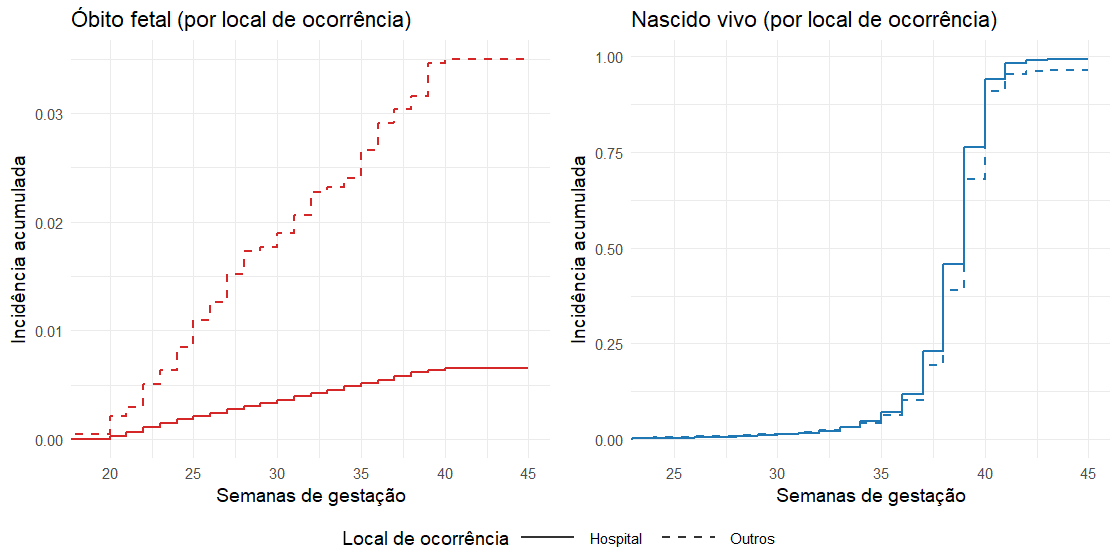
\includegraphics[width=0.9\linewidth]{figuras/cif_lococornasc_painel_ambos.png}
  \fonte{Fonte: figura feita pelo autor.}
  \label{fig:cif_lococornasc_painel_ambos}
\end{figure}

Assim, o local de ocorrência sugere maior acúmulo de óbitos fetais fora do
hospital, mas essa conclusão deve ser vista como exploratória. A baixa frequência
da categoria "Outros" limita a estabilidade da comparação e impede uma leitura
mais forte sobre diferenças.

%---------------------------------------------------------
%---------------------- sexo
%---------------------------------------------------------

%---------------------- KM
Nos gráficos de Kaplan-Meier da Figura \ref{fig:ambos_KM_sexo}, as curvas por
sexo do recém-nascido permanecem bastante próximas. Ainda assim, pelo tamanho da
base, o Log-rank identificou diferença estatística tanto para óbito fetal
($\chi^2=6{,}77$; $p<0{,}01$) quanto para nascimento vivo ($\chi^2=110$;
$p<0{,}001$). Dentro de cada desfecho, porém, as medianas foram iguais entre
meninos e meninas: 29 semanas (24--35) para ambos nos óbitos fetais e 39 semanas (38--39)
nos nascidos vivos. Como complemento, as médias $\pm$ DP (mediana) foram de 29,30
$\pm$ 6,37 (29) no sexo masculino e 29,50 $\pm$ 5,97 (29) no feminino entre os
óbitos fetais, e de 38,22 $\pm$ 2,16 (39) e 38,29 $\pm$ 2,10 (39) entre os
nascidos vivos. Por tanto, é notável que a diferença é pequena em termos
práticos.
\begin{figure}[H]
  \centering
  \caption{Gráficos de Kaplan-Meier da variável sexo para cada desfecho.}
  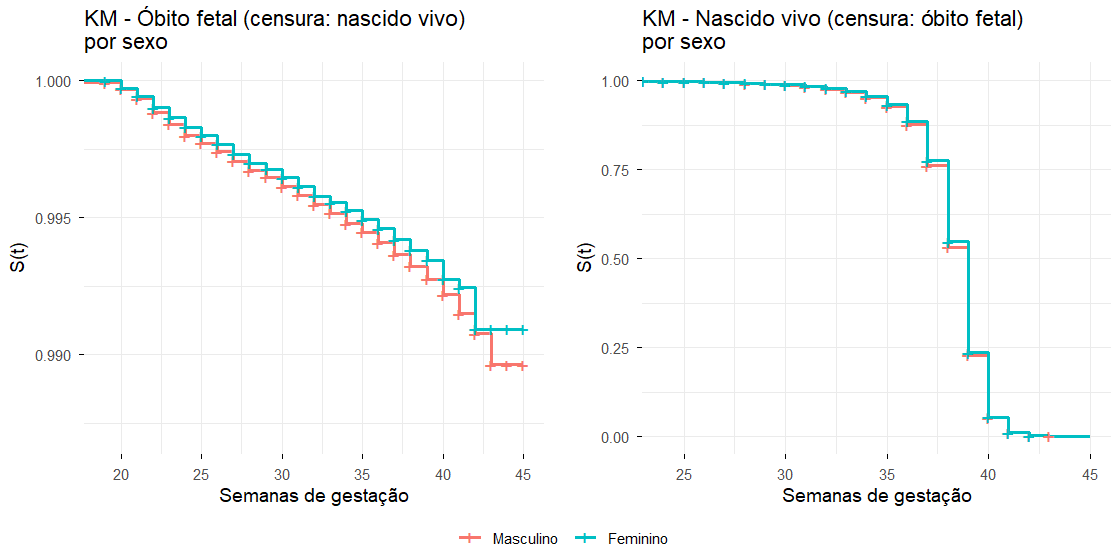
\includegraphics[width=0.9\linewidth]{figuras/kmglobal_sexo.png}
  \fonte{Fonte: figura feita pelo autor.}
  \label{fig:ambos_KM_sexo}
\end{figure}
%---------------------- CIF
Na Figura \ref{fig:ambos_cif_sexo}, as diferenças permaneceram pequenas nas
curvas de incidência acumulada. Entre os óbitos fetais, o sexo masculino teve
frequência um pouco maior (53,2\%) e CIF discretamente superior ao longo do
acompanhamento, chegando a 0,69\% na semana 40, contra 0,63\% no sexo feminino.
O teste de Gray para óbito fetal foi significativo ($\chi^2=6{,}14$; $p=0{,}013$).
Entre os nascidos vivos, as curvas ficaram muito próximas em todo o período, com
CIF de 94,07\% para meninos e 93,93\% para meninas na semana 40, apesar do teste de Gray ser 
significativo ($\chi^2=750\,287$; $p<0{,}001$). Por tanto, a evidência estatística
existe, mas a magnitude absoluta da diferença foi pequena.
\begin{figure}[H]
  \centering
  \caption{Gráficos de incidência acumulada da variável sexo para cada desfecho.}
  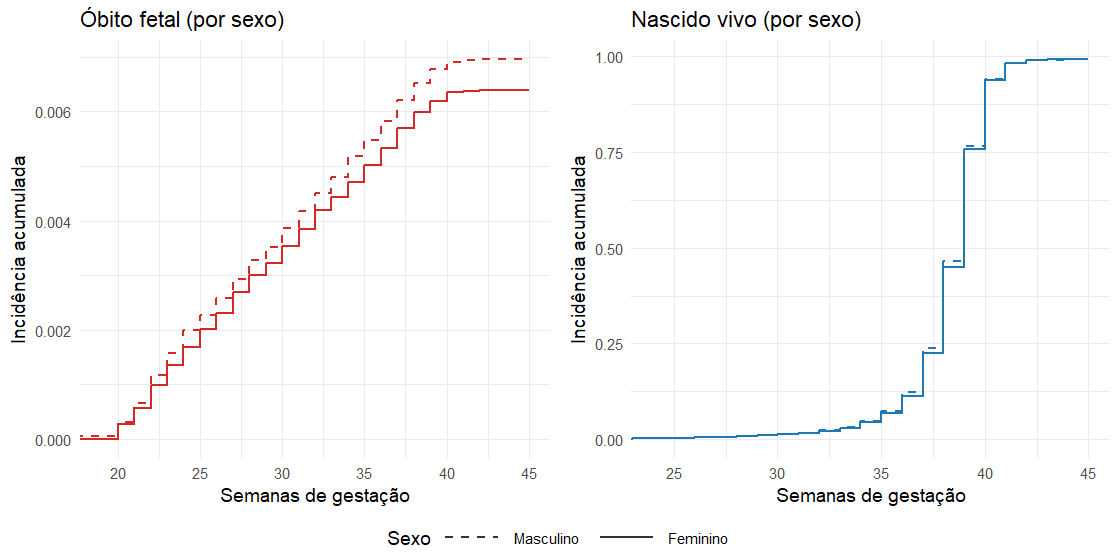
\includegraphics[width=0.9\linewidth]{figuras/ambos_cif_sexo.png}
  \fonte{Fonte: figura feita pelo autor.}
  \label{fig:ambos_cif_sexo}
\end{figure}

Assim, o sexo do recém-nascido apresentou diferenças estatísticas, mas com
pequena importância prática nesta análise. As curvas, medianas e CIF ficaram
muito próximas, indicando que essa variável não foi uma das principais fontes de
diferença no tempo até os desfechos.

Em geral, os resultados das variáveis em comum nas bases de dados mostram que tipo de gestação,
faixa de peso ao nascer e tipo de parto foram os fatores que mais diferenciaram o
tempo até o desfecho. Escolaridade materna, idade materna e antecedente de filhos
mortos também apresentaram contraste relevante, embora menor. Já sexo e presença
de filhos vivos previamente tiveram diferenças pequenas em termos absolutos, e o
local de ocorrência do parto deve ser interpretado com cautela devido ao pequeno
número de registros fora do hospital.

\section{Variáveis exclusivas de cada causa}

A Tabela \ref{tab:tabela-descritiva-exclusivas} reúne as medidas descritivas das
variáveis disponíveis exclusivamente em uma das bases de dados e serve como ponto de partida para 
a leitura dos gráficos de Kaplan-Meier apresentados a seguir.

%---------------- Tabela das variáveis exclusivas
\newpage
\begin{table}[H]
\centering
\renewcommand{\arraystretch}{1.0}
\caption{Medidas descritivas das variáveis exclusivas de cada causa.}
\begin{tabular}{@{}p{0.32\textwidth} p{0.42\textwidth} p{0.16\textwidth}@{}}
\specialrule{0.16em}{0pt}{0pt}
\textbf{Variáveis numéricas} & \textbf{Média $\pm$ DP} & \textbf{Base de dados} \\
\specialrule{0.16em}{0pt}{0pt}
Apgar no 5º minuto (apgar5)                 & 9,41 $\pm$ 0,85   & SINASC \\
Mês de início do pré-natal (mesprenat)     & 2,22 $\pm$ 1,23   & SINASC \\
Nº total de gestações prévias (qtdgestant) & 1,20 $\pm$ 1,36   & SINASC \\
Nº de partos vaginais prévios (qtdpartnor) & 0,55 $\pm$ 1,04   & SINASC \\
Nº de partos cesáreos prévios (qtdpartces) & 0,41 $\pm$ 0,74   & SINASC \\
\specialrule{0.16em}{6pt}{0pt}

\textbf{Variáveis categóricas} & \textbf{Categoria: n (\%)} & \textbf{Base de dados} \\
\specialrule{0.16em}{0pt}{0pt}

Momento do óbito em relação ao parto (obitoparto) &
\begin{tabular}{@{}l@{}}
Antes: 3\,107 (95,1\,\%)\\[-2pt]
Durante: 159 (4,9\,\%)
\end{tabular} &
SIM--DOFET \\
\hline

Apgar no 5º minuto (apgar5) &
\begin{tabular}{@{}l@{}}
$> 7$: 476\,794 (98,1\,\%)\\[-2pt]
$\leq 7$: 9\,128 (1,9\,\%)
\end{tabular} &
SINASC \\
\hline

Consultas de pré-natal (consultas) &
\begin{tabular}{@{}l@{}}
Nenhuma: 468 (0,1\,\%)\\[-2pt]
De 1 a 3: 15\,526 (3,2\,\%)\\[-2pt]
De 4 a 6: 63\,648 (13,1\,\%)\\[-2pt]
7 e mais: 406\,280 (83,6\,\%)
\end{tabular} &
SINASC \\
\hline

Anomalia identificada (idanomal) &
\begin{tabular}{@{}l@{}}
Sim: 7\,550 (1,6\,\%)\\[-2pt]
Não: 478\,372 (98,4\,\%)
\end{tabular} &
SINASC \\
\hline

Início do pré-natal (mesprenat) &
\begin{tabular}{@{}l@{}}
Primeiro trimestre: 432\,864 (89,1\,\%)\\[-2pt]
Segundo trimestre: 46\,020 (9,5\,\%)\\[-2pt]
Terceiro trimestre: 7\,038 (1,4\,\%)
\end{tabular} &
SINASC \\
\hline

Paridade (paridade) &
\begin{tabular}{@{}l@{}}
Nulípara: 184\,346 (37,9\,\%)\\[-2pt]
Multípara: 301\,576 (62,1\,\%)
\end{tabular} &
SINASC \\
\hline

Gestações prévias (qtdgestant) &
\begin{tabular}{@{}l@{}}
Não: 184\,858 (38,0\,\%)\\[-2pt]
Sim: 301\,064 (62,0\,\%)
\end{tabular} &
SINASC \\
\hline

Partos cesáreos prévios (qtdpartces) &
\begin{tabular}{@{}l@{}}
Não: 338\,498 (69,7\,\%)\\[-2pt]
Sim: 147\,424 (30,3\,\%)
\end{tabular} &
SINASC \\
\hline

Partos vaginais prévios (qtdpartnor) &
\begin{tabular}{@{}l@{}}
Não: 333\,278 (68,6\,\%)\\[-2pt]
Sim: 152\,644 (31,4\,\%)
\end{tabular} &
SINASC \\
\hline

Raça/cor da mãe (racacormae) &
\begin{tabular}{@{}l@{}}
Branca: 255\,439 (52,6\,\%)\\[-2pt]
Preta: 39\,259 (8,1\,\%)\\[-2pt]
Amarela: 2\,566 (0,5\,\%)\\[-2pt]
Parda: 188\,113 (38,7\,\%)\\[-2pt]
Indígena: 545 (0,1\,\%)
\end{tabular} &
SINASC \\
\hline

Cesárea antes do trabalho de parto (stcesparto) &
\begin{tabular}{@{}l@{}}
Sim: 198\,839 (40,9\,\%)\\[-2pt]
Não: 97\,723 (20,1\,\%)\\[-2pt]
Não se aplica: 189\,360 (39,0\,\%)
\end{tabular} &
SINASC \\
\hline

Trabalho de parto induzido (sttrabpart) &
\begin{tabular}{@{}l@{}}
Sim: 95\,508 (19,7\,\%)\\[-2pt]
Não: 390\,414 (80,3\,\%)
\end{tabular} &
SINASC \\
\specialrule{0.16em}{0pt}{0pt}
\end{tabular}
\fonte{Média $\pm$ DP (desvio padrão) das variáveis numéricas. n (\%): frequências em
relação ao total de indivíduos de cada grupo. Fonte: elaboração do autor.}
\label{tab:tabela-descritiva-exclusivas}
\end{table}

%---------------------------------------------------------
%---------------------- momento do óbito (em relação ao parto)
%---------------------------------------------------------

Na Figura \ref{fig:km_obitos_obitoparto}, as curvas de Kaplan-Meier sugerem que
o momento do óbito em relação ao parto distingue o tempo até o desfecho. Os
óbitos classificados como ocorridos durante o parto se concentraram em idades
gestacionais mais precoces, com mediana de 24 semanas (22--33), enquanto os
óbitos anteriores ao parto apresentaram mediana de 30 semanas (24--35). O teste
de Log-rank indicou diferença estatística
($\chi^2=7{,}22$; $p=0{,}007$). Ainda assim, a grande maioria dos registros
correspondeu a óbitos anteriores ao parto (95,1\%), como mostra a Tabela
\ref{tab:tabela-descritiva-exclusivas}.
\begin{figure}[H]
  \centering
  \caption{Gráfico de Kaplan-Meier da variável obitoparto referente ao momento do óbito em
  relação ao parto.}
  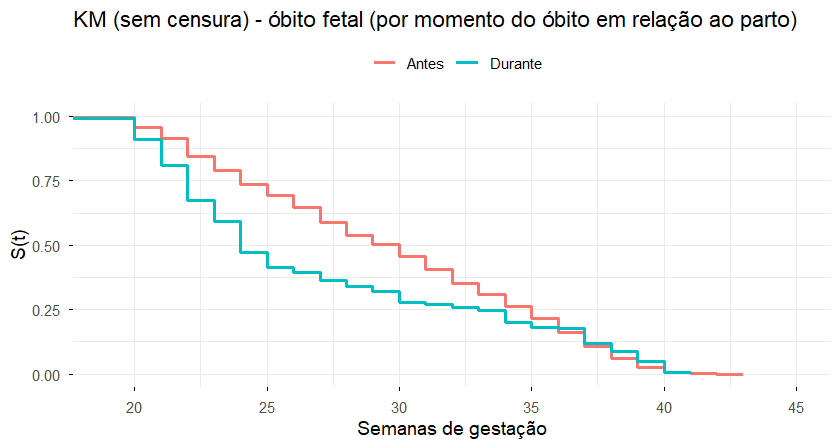
\includegraphics[width=0.9\linewidth]{figuras/km_obitos_obitoparto.png}
  \fonte{Fonte: figura feita pelo autor.}
  \label{fig:km_obitos_obitoparto}
\end{figure}

Assim, embora a maioria dos óbitos fetais tenha ocorrido antes do parto, os poucos 
casos classificados como ocorridos durante o parto aconteceram, em média/mediana, em 
idades gestacionais mais precoces. Portanto, essas categorias parecem representar 
situações obstétricas diferentes dentro dos óbitos fetais, identificando subgrupos 
distintos.

%---------------------------------------------------------
%---------------------- apgar5
%---------------------------------------------------------

Na Figura \ref{fig:km_nascidosvivos_apgar}, as curvas de Kaplan-Meier sugerem, em 
um primeiro momento, diferença entre as curvas. Entre os nascidos vivos, recém nascidos 
com Apgar no quinto minuto igual ou inferior a 7 apresentaram partos em idades
gestacionais menores. Nesse grupo, a mediana foi de 37 semanas (32--39), contra 
39 semanas (38--39) no grupo com Apgar acima de 7. O Log-rank foi 
significativo ($\chi^2=3\,781$; $p<0{,}001$). Embora esse contraste seja nítido, o Apgar 
é medido após o nascimento. Portanto, esse resultado deve ser entendido como marcador de 
pior condição neonatal associado à prematuridade, e não como fator anterior ao tempo 
até o parto.
\begin{figure}[H]
  \centering
  \caption{Gráfico de Kaplan-Meier da variável apgar5 referente ao índice de Apgar no quinto
  minuto.}
  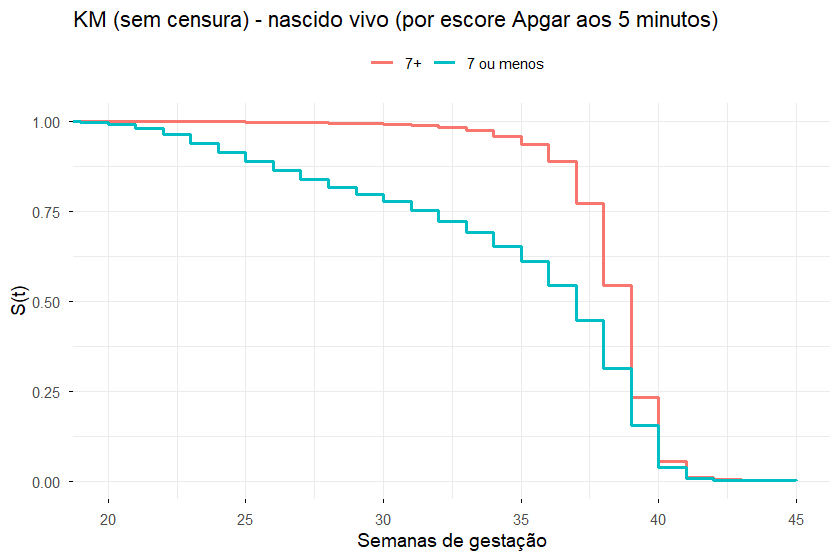
\includegraphics[width=0.9\linewidth]{figuras/km_nascidosvivos_apgar.png}
  \fonte{Fonte: figura feita pelo autor.}
  \label{fig:km_nascidosvivos_apgar}
\end{figure}

No geral, o Apgar no quinto minuto resume um contraste clínico importante entre
os nascidos vivos. Valores menores ou iguais a 7 estiveram ligados a partos mais
precoces e a pior condição neonatal imediata, funcionando mais como marcador do
estado do recém-nascido do que como variável anterior ao parto.

%---------------------------------------------------------
%---------------------- Número de consultas pré-natal
%---------------------------------------------------------

Na Figura \ref{fig:km_nascidosvivos_consultas}, as curvas de Kaplan-Meier
sugerem diferenças mais claras segundo o número de consultas pré-natais. No
grupo com 7 ou mais consultas, a mediana foi de 39 semanas (38--39). Nos grupos
com nenhuma, de 1 a 3 e de 4 a 6 consultas, as medianas foram de 38 semanas, com
intervalos interquartílicos de 37--39, 36--39 e 37--39, respectivamente. O
Log-rank foi significativo ($\chi^2=6\,412$; $p<0{,}001$).
\begin{figure}[H]
  \centering
  \caption{Gráfico de Kaplan-Meier da variável consultas referente ao número de consultas
  pré-natal.}
  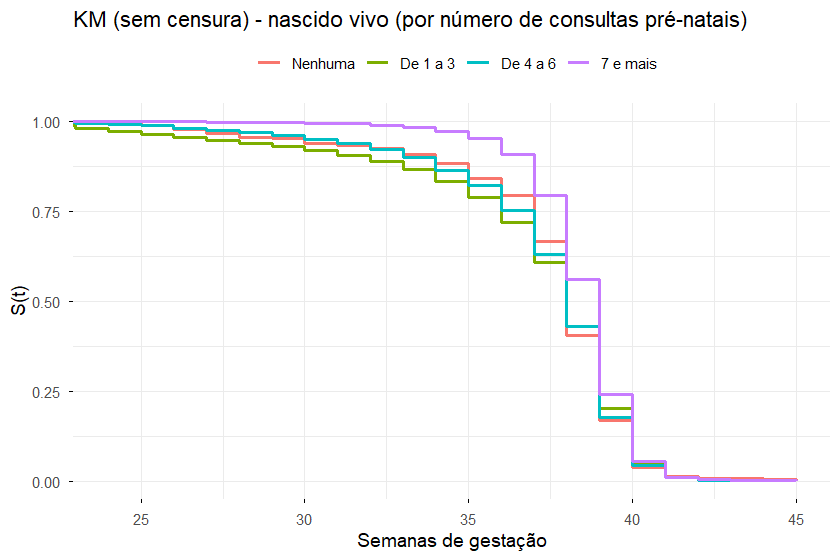
\includegraphics[width=0.9\linewidth]{figuras/km_nascidosvivos_consultas.png}
  \fonte{Fonte: figura feita pelo autor.}
  \label{fig:km_nascidosvivos_consultas}
\end{figure}

Por tanto, o número de consultas pré-natais diferenciou ligeiramente o tempo até o
nascimento vivo, com partos mais precoces entre gestações com menor número de
consultas. Partos prematuros deixam menos tempo para a gestante realizar várias 
consultas. Então, a associação entre poucas consultas e parto mais precoce pode 
refletir tanto falhas de acompanhamento quanto a própria menor duração da 
gestação. Por isso, não devemos concluir automaticamente que mais consultas, sozinhas, 
causam partos mais tardios. Além disso, embora tenha sido detectado diferença entre as 
curvas através do Log-Rank, a diferença em magnitude é sutil.


%---------------------------------------------------------
%---------------------- Anomalia identificada
%---------------------------------------------------------

Na Figura \ref{fig:km_nascidosvivos_anomalia}, as curvas de Kaplan-Meier não sugerem
uma diferença muito clara entre as curvas. Porém, a presença de anomalia identificada 
parece se associar a partos mais precoces. O grupo com anomalia apresentou mediana de 
38 semanas (37--39), contra 39 semanas (38--39) na ausência de anomalia. O Log-rank foi 
significativo ($\chi^2=605$; $p<0{,}001$).
\begin{figure}[H]
  \centering
  \caption{Gráfico de Kaplan-Meier da variável idanomal referente a anomalia identificada.}
  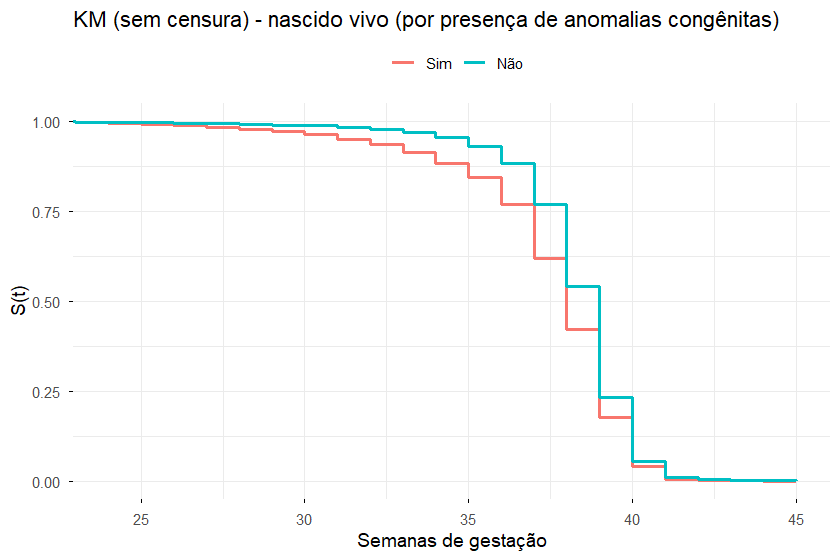
\includegraphics[width=0.9\linewidth]{figuras/km_nascidosvivos_anomalia.png}
  \fonte{Fonte: figura feita pelo autor.}
  \label{fig:km_nascidosvivos_anomalia}
\end{figure}

Por tanto, há algum indício de que a presença de anomalia identificada esteve 
associada a nascimentos em idades gestacionais menores. Esse resultado sugere 
um grupo de maior complexidade clínica, possivelmente relacionado tanto à condição 
fetal quanto a decisões assistenciais de interrupção mais precoce.

%---------------------------------------------------------
%---------------------- Mês de gestação em que se iniciou o pré-natal
%---------------------------------------------------------

Na Figura \ref{fig:km_nascidosvivos_mesprenat}, as curvas de Kaplan-Meier
sugerem diferença segundo o trimestre de início do pré-natal, embora as medianas
tenham permanecido em 39 semanas em todos os grupos. O intervalo interquartílico
foi de 38--39 para início no primeiro trimestre e de 38--40 para início no
segundo e no terceiro. Como complemento, as médias $\pm$ DP (mediana) foram de
38,26 $\pm$ 2,11 (39), 38,19 $\pm$ 2,37 (39) e 38,32 $\pm$ 1,93 (39),
respectivamente. O Log-rank foi significativo ($\chi^2=70{,}90$; $p<0{,}001$),
mas a principal diferença foi pequena e sugere partos ligeiramente mais precoces
entre mulheres que iniciaram o acompanhamento no segundo trimestre. Como o grupo
com início no terceiro trimestre foi bem menor, essa interpretação deve ser
feita com cautela.
\begin{figure}[H]
  \centering
  \caption{Gráfico de Kaplan-Meier da variável mesprenat referente ao mês de gestação em que
  se iniciou o pré-natal.}
  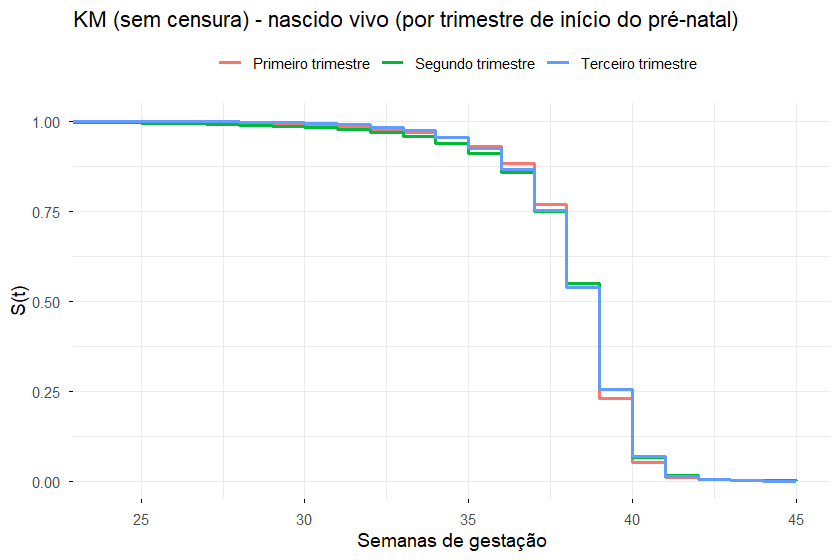
\includegraphics[width=0.9\linewidth]{figuras/km_nascidosvivos_mesprenat.png}
  \fonte{Fonte: figura feita pelo autor.}
  \label{fig:km_nascidosvivos_mesprenat}
\end{figure}

Assim, o trimestre de início do pré-natal mostrou diferença estatística, mas com
pequena magnitude na escala de semanas. Por tanto, essa variável deve ser lida 
como parte do contexto de acesso e acompanhamento da gestação, sem indicar, 
isoladamente, grande mudança no tempo até o nascimento.

%---------------------------------------------------------
%---------------------- Paridade
%---------------------------------------------------------

Na Figura \ref{fig:km_nascidosvivos_paridade}, as curvas de Kaplan-Meier sugerem
diferença discreta segundo a paridade. A mediana foi de 39 semanas nos dois
grupos, com intervalo interquartílico de 38--40 nas nulíparas e 38--39 nas
multíparas. Como complemento, as médias $\pm$ DP (mediana) foram de 38,34
$\pm$ 2,20 (39) e 38,20 $\pm$ 2,08 (39), respectivamente. O Log-rank foi
significativo ($\chi^2=1\,618$; $p<0{,}001$), mas a magnitude absoluta dessa
diferença foi pequena.
\begin{figure}[H]
  \centering
  \caption{Gráfico de Kaplan-Meier da variável paridade referente a se é a primeira gravidez
  ou se teve mais de uma.}
  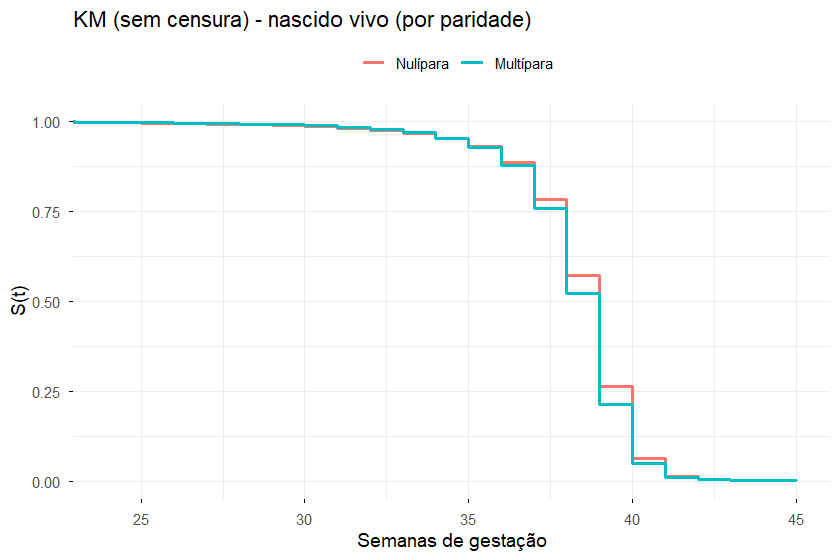
\includegraphics[width=0.9\linewidth]{figuras/km_nascidosvivos_paridade.png}
  \fonte{Fonte: figura feita pelo autor.}
  \label{fig:km_nascidosvivos_paridade}
\end{figure}

No geral, a paridade apresentou diferença detectável, mas discreta. A condição
de nulípara ou multípara, isoladamente, não pareceu modificar de forma importante
o tempo gestacional até o nascimento vivo nesta análise.

%---------------------------------------------------------
%---------------------- Número total de gestações anteriores
%---------------------------------------------------------

Na Figura \ref{fig:km_nascidosvivos_qtdgestant}, as curvas de Kaplan-Meier
sugerem diferença segundo a presença de gestações anteriores, embora com pequena
magnitude. A mediana foi de 39 semanas nos dois grupos, com Q1--Q3 de 38--40 nas
mulheres sem gestações prévias e 38--39 naquelas com história gestacional prévia.
Como complemento, as médias $\pm$ DP (mediana) foram de 38,34 $\pm$ 2,20 (39) e
38,20 $\pm$ 2,08 (39), respectivamente. O Log-rank foi significativo
($\chi^2=1\,614$; $p<0{,}001$), mas a diferença absoluta foi pequena.
\begin{figure}[H]
  \centering
  \caption{Gráfico de Kaplan-Meier da variável qtdgestant referente ao número total de
  gestações anteriores.}
  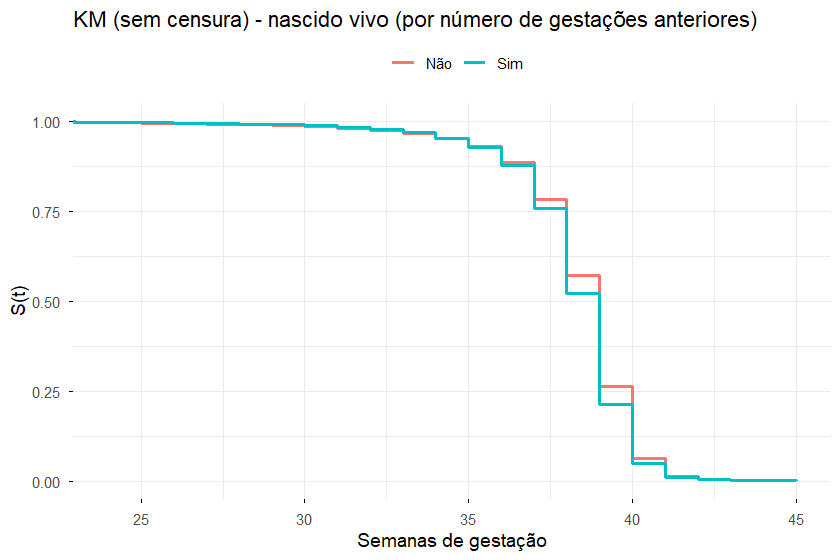
\includegraphics[width=0.9\linewidth]{figuras/km_nascidosvivos_qtdgestant.png}
  \fonte{Fonte: figura feita pelo autor.}
  \label{fig:km_nascidosvivos_qtdgestant}
\end{figure}

De forma semelhante à paridade, a presença de gestações anteriores indicou
diferença estatística pequena. O resultado sugere que o histórico gestacional
prévio, quando avaliado apenas por essa categorização, teve pouca expressão
prática sobre a idade gestacional ao nascimento.

%---------------------------------------------------------
%---------------------- Número total de partos cesáreos anteriores
%---------------------------------------------------------

Na Figura \ref{fig:km_nascidosvivos_qtdpartces}, as curvas de Kaplan-Meier não 
deixam evidente se existe diferença significativa, mas há indícios de que o 
histórico de cesarianas prévias esteve associada a partos discretamente mais 
precoces. Mulheres com cesariana anterior apresentaram mediana de 38 
semanas (38--39), contra 39 semanas (38--40) nas demais. O Log-rank foi 
significativo ($\chi^2=3\,071$; $p<0{,}001$).
\begin{figure}[H]
  \centering
  \caption{Gráfico de Kaplan-Meier da variável qtdpartces referente ao número total de
  partos cesáreos anteriores.}
  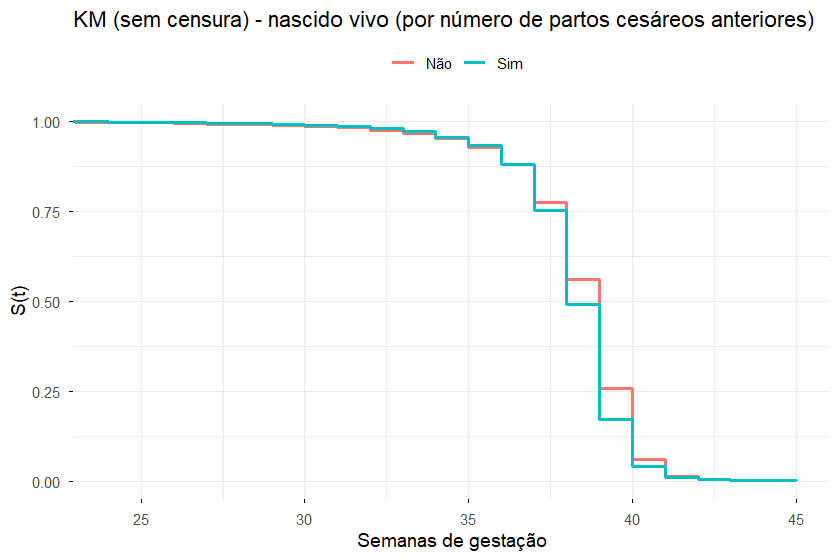
\includegraphics[width=0.9\linewidth]{figuras/km_nascidosvivos_qtdpartces.png}
  \fonte{Fonte: figura feita pelo autor.}
  \label{fig:km_nascidosvivos_qtdpartces}
\end{figure}

Assim, há indícios de que o histórico de cesariana anterior se associa a nascimentos um pouco
mais precoces.

%---------------------------------------------------------
%---------------------- Número total de de partos vaginais anteriores.
%---------------------------------------------------------

Na Figura \ref{fig:km_nascidosvivos_qtdpartnor}, as curvas de Kaplan-Meier
sugerem pouca diferença segundo o número de partos vaginais anteriores. O teste
de Log-rank foi significativo ($\chi^2=46{,}74$; $p<0{,}001$), mas as medianas
foram de 39 semanas em ambos os grupos, com Q1--Q3 de 38--39. As médias $\pm$ DP
(mediana) praticamente coincidiram: 38,26 $\pm$ 2,12 (39) entre mulheres sem
partos vaginais prévios e 38,25 $\pm$ 2,16 (39) entre aquelas com esse
antecedente. Isso sugere pouca relevância clínica nessa diferença.
\begin{figure}[H]
  \centering
  \caption{Gráfico de Kaplan-Meier da variável qtdpartnor referente ao número total de
  partos vaginais anteriores.}
  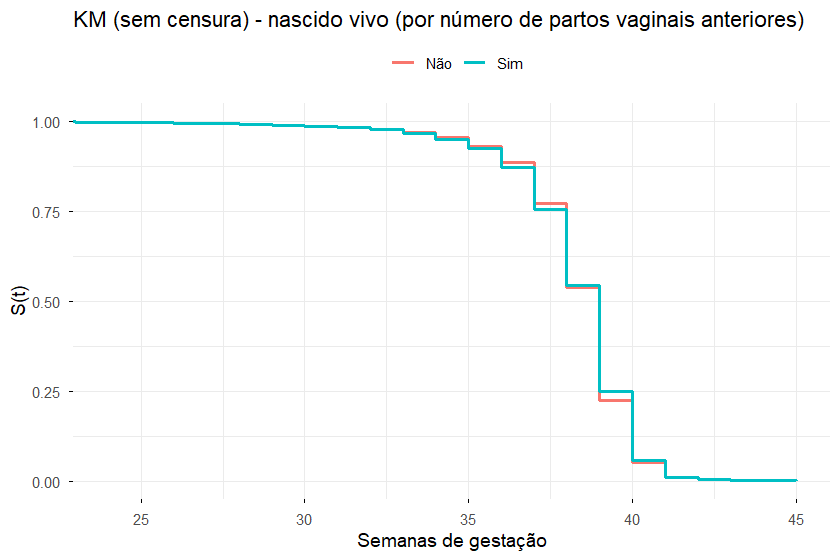
\includegraphics[width=0.9\linewidth]{figuras/km_nascidosvivos_qtdpartnor.png}
  \fonte{Fonte: figura feita pelo autor.}
  \label{fig:km_nascidosvivos_qtdpartnor}
\end{figure}

Por tanto, o número de partos vaginais anteriores apresentou pouca contribuição para
diferenciar a idade gestacional ao nascimento. Apesar da significância
estatística, as medidas descritivas praticamente coincidiram entre os grupos.

%---------------------------------------------------------
%---------------------- Raça/cor da mãe
%---------------------------------------------------------

Na Figura \ref{fig:km_nascidosvivos_racamae}, as curvas de Kaplan-Meier sugerem
diferença estatística global para raça/cor da mãe, mas com curvas bastante
próximas e mediana de 39 semanas em todos os grupos. O Log-rank foi significativo
($\chi^2=943$; $p<0{,}001$). Os intervalos interquartílicos foram muito
próximos: 38--39 em brancas e amarelas e 38--40 em pretas, pardas e indígenas.
Como complemento, as médias $\pm$ DP (mediana) variaram pouco, de 38,22
$\pm$ 2,07 (39) entre brancas a 38,51 $\pm$ 1,83 (39) entre indígenas. Assim,
embora exista heterogeneidade detectável, sua magnitude prática foi pequena
nesta análise descritiva, especialmente diante do grande tamanho amostral e do
baixo número de observações em algumas categorias, como indígenas e amarelas.
\begin{figure}[H]
  \centering
  \caption{Gráfico de Kaplan-Meier da variável racacormae referente a raça/cor da mãe.}
  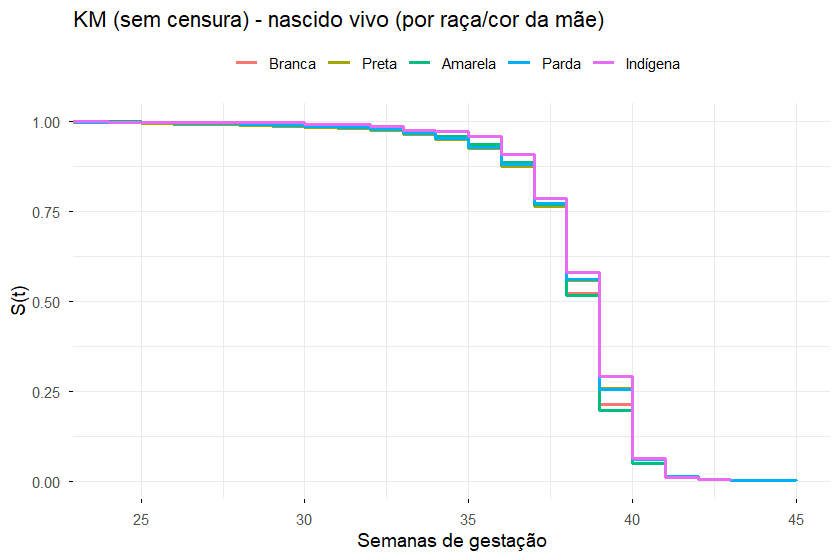
\includegraphics[width=0.9\linewidth]{figuras/km_nascidosvivos_racamae.png}
  \fonte{Fonte: figura feita pelo autor.}
  \label{fig:km_nascidosvivos_racamae}
\end{figure}

No geral, raça/cor materna mostrou heterogeneidade estatística, mas sem grande
separação prática das curvas.

%---------------------------------------------------------
%---------------------- Cesárea ocorreu antes do trabalho de parto iniciar
%---------------------------------------------------------

Na Figura \ref{fig:km_nascidosvivos_stcesparto}, as curvas de Kaplan-Meier
sugerem separação nítida para a variável referente à cesariana antes do início do
trabalho de parto. Os nascimentos com cesariana programada tiveram mediana de 38
semanas (37--39), enquanto as categorias ``não'' e ``não se aplica'' apresentaram
mediana de 39 semanas, com Q1--Q3 de 38--39 e 38--40, respectivamente. O
Log-rank foi significativo ($\chi^2=5\,319$; $p<0{,}001$).
\begin{figure}[H]
  \centering
  \caption{Gráfico de Kaplan-Meier da variável stcesparto referente a se cesária ocorreu
  antes do trabalho de parto iniciar.}
  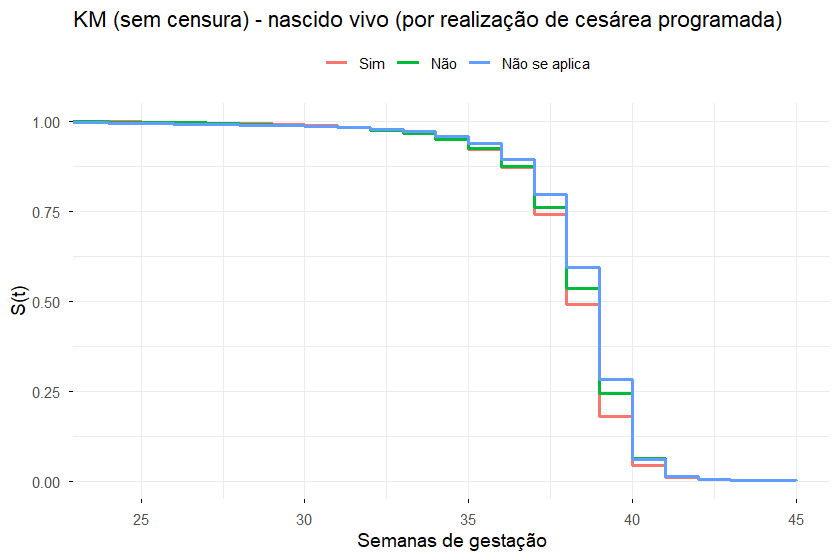
\includegraphics[width=0.9\linewidth]{figuras/km_nascidosvivos_stcesparto.png}
  \fonte{Fonte: figura feita pelo autor.}
  \label{fig:km_nascidosvivos_stcesparto}
\end{figure}

Assim, para a cesariana antes do início do trabalho de parto, há indício de 
associação a nascimentos mais precoces.

%---------------------------------------------------------
%---------------------- Trabalho de parto induzido
%---------------------------------------------------------

Na Figura \ref{fig:km_nascidosvivos_indtrabalhoparto}, embora não é claro se as curvas de
Kaplan-Meier sugerem diferenças, há indícios de que a indução do trabalho de parto esteve 
associada a nascimentos em idades gestacionais mais avançadas. A mediana foi de 39 
semanas nos dois grupos, mas o intervalo interquartílico foi de 38--40 no grupo com
indução e 38--39 no grupo sem indução. Como complemento, as médias $\pm$ DP
(mediana) foram de 38,72 $\pm$ 1,77 (39) e 38,14 $\pm$ 2,19 (39),
respectivamente. O Log-rank foi significativo ($\chi^2=7\,046$; $p<0{,}001$).
Esse padrão sugere que, nesta base, a indução ocorreu com mais frequência 
(embora discretamente) em gestações que chegaram ao termo ou ao pós-termo.
\begin{figure}[H]
  \centering
  \caption{Gráfico de Kaplan-Meier da variável sttrabpart referente a trabalho de parto
  induzido.}
  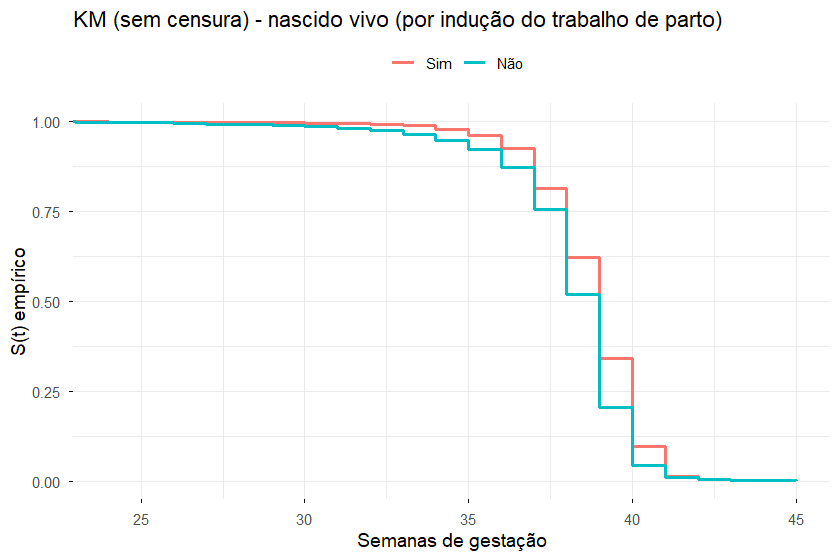
\includegraphics[width=0.9\linewidth]{figuras/km_nascidosvivos_indtrabalhoparto.png}
  \fonte{Fonte: figura feita pelo autor.}
  \label{fig:km_nascidosvivos_indtrabalhoparto}
\end{figure}

Assim, há indícios de que a indução do trabalho de parto está discretamente associada a 
idades gestacionais mais avançadas. Houve diferença estatística e um deslocamento leve 
para idades gestacionais mais avançadas no grupo com indução, mas a magnitude foi 
pequena, o que pode estar refletindo uma conduta assistencial aplicada em momento 
mais tardio da gestação.

No geral, as variáveis exclusivas reforçam alguns pontos importantes. Nos
óbitos fetais, o momento do óbito em relação ao parto foi a única variável
exclusiva disponível a sugerir diferença no tempo até o desfecho, com mediana de
24 semanas (22--33) nos casos ocorridos durante o parto e de 30 semanas (24--35)
nos anteriores ao parto. Nos nascidos vivos, a maior parte das variáveis manteve
mediana de 39 semanas, de modo que muitos resultados estatisticamente
significativos devem ser
lidos como diferenças pequenas na escala das semanas. Os contrastes com maior
relevância prática apareceram no Apgar no quinto minuto, nas consultas de
pré-natal, na cesariana antes do trabalho de parto e na presença de anomalia
identificada. Esses resultados são coerentes com situações relacionadas à
prematuridade, à organização da assistência obstétrica e às condições do
recém-nascido, embora não devam ser interpretados isoladamente como relações
causais.

\section{Redes Regionais de Atenção à Saúde (RRAS)}

A Figura \ref{fig:mapas_RRAS} apresenta dois mapas do estado de São Paulo segundo
a divisão em 18 RRAS adotada nesta análise, mostrando a participação percentual
de óbitos fetais e de nascidos vivos no total estadual. Esses percentuais devem
ser lidos como distribuição do volume de eventos, e não como risco individual,
pois regiões mais populosas tendem naturalmente a concentrar mais registros. Em
ambos os mapas, a RRAS 6 concentrou as maiores proporções, com 23,79\% dos
óbitos fetais e 26,15\% dos nascidos vivos, resultado compatível com sua densidade 
populacional. Fora da RRAS 6, a participação de óbitos fetais foi
mais alta nas RRAS 2 (10,96\%), 15 (7,10\%), 7 (6,00\%), 8 (5,21\%), 5
(4,99\%), 13 (4,99\%) e 17 (4,96\%). Para os nascidos vivos, destacaram-se as
RRAS 15 (8,76\%), 2 (7,56\%), 8 (6,15\%), 17 (5,52\%), 13 (5,49\%), 1 (5,40\%)
e 5 (5,13\%).

\begin{figure}[H]
  \centering
  \caption{Mapas do estado de São Paulo por RRAS identificando a contribuição de
  óbitos fetais e de nascidos vivos de cada RRAS em relação ao total estadual.}
  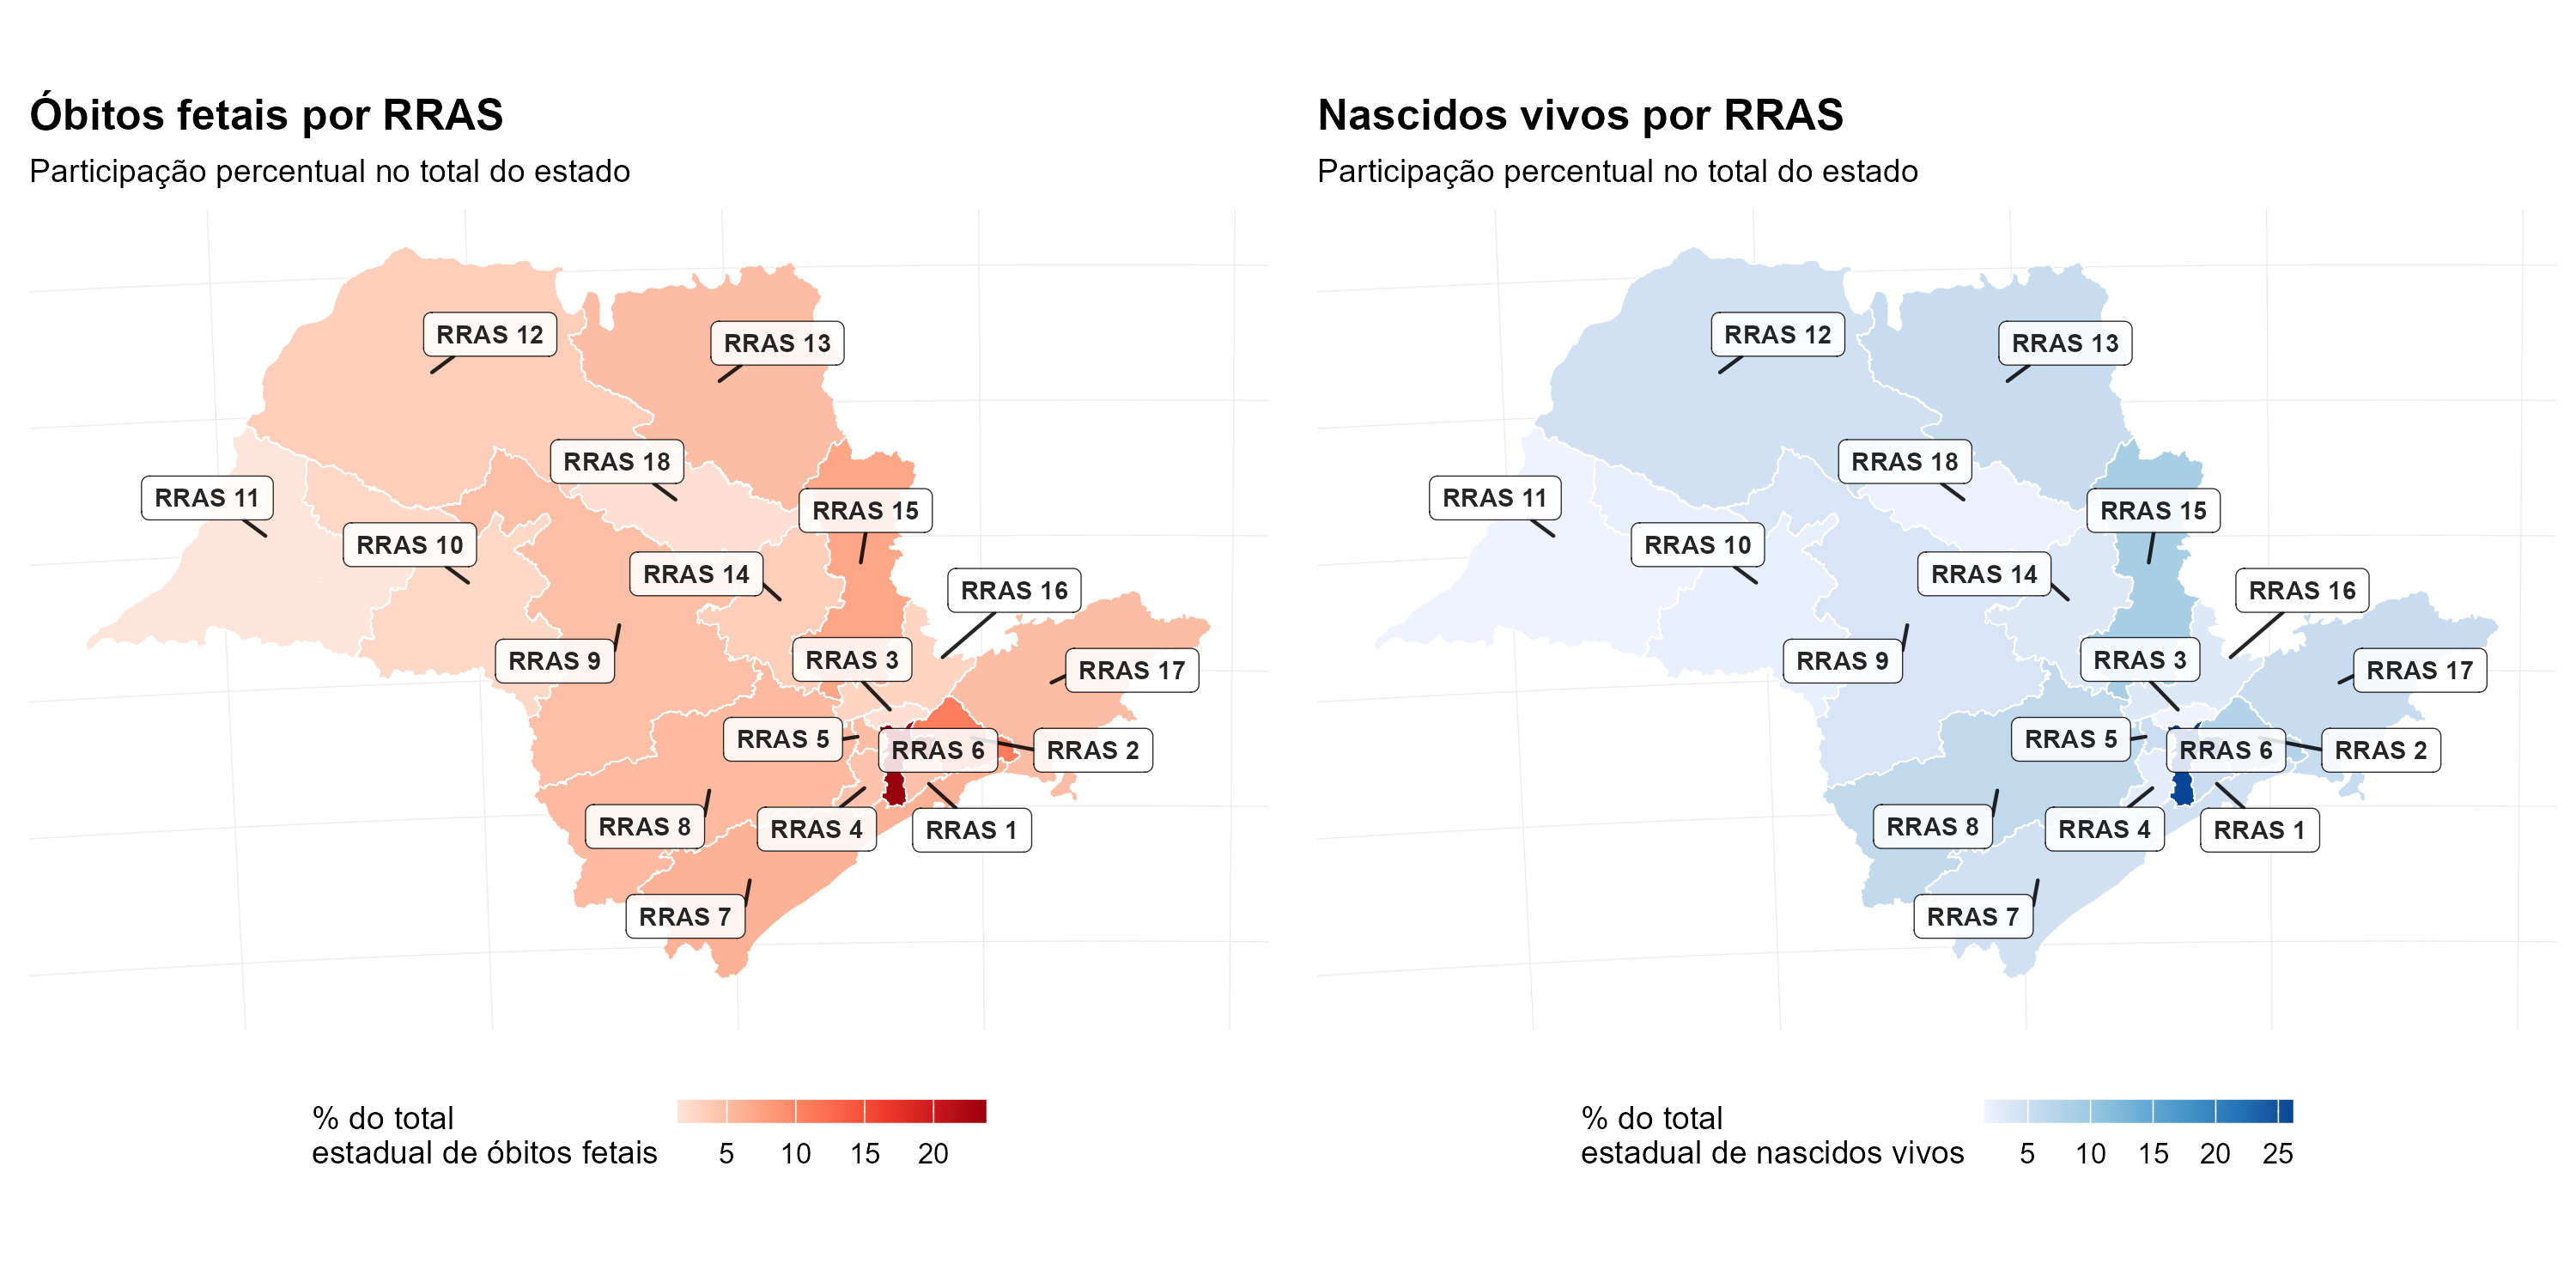
\includegraphics[width=0.9\linewidth]{figuras/mapas_RRAS.png}
  \fonte{Fonte: elaboração do autor.}
  \label{fig:mapas_RRAS}
\end{figure}

A Tabela \ref{tab:indicadores-rras-compacta} detalha os valores absolutos,
percentuais, taxas e prematuridade por RRAS. A maior taxa de óbitos fetais por 
1000 nascidos vivos foi observada na RRAS 4, com 10,65 óbitos fetais, seguida 
pelas RRAS 2 (9,74), 7 (8,85), 3 (8,65) e 9 (8,32). Assim, o maior número absoluto 
de óbitos fetais não coincidiu necessariamente com a maior taxa: embora a RRAS 6 
tenha concentrado 777 óbitos fetais, sua taxa foi de 6,12 por 1000 nascidos vivos. 
A RRAS 15 também reuniu número absoluto alto de óbitos fetais (232), mas com taxa mais
baixa, de 5,45 por 1000 nascidos vivos.

Entre os nascidos vivos, a RRAS 6 também liderou em número absoluto, com
127.062 registros (26,15\%). Além disso, as maiores taxas de nascidos vivos por 1000 habitantes 
foram observadas nas RRAS 5 (12,01), 2 (11,83), 4 (11,52), 3 (11,47), 8 (11,36) 
e 16 (11,36). Em contraste, as menores taxas ocorreram nas RRAS 12 (9,26), 18 (9,35) 
e 1 (9,62). Esse padrão mostra que a participação no total estadual reflete 
principalmente o tamanho populacional, enquanto as taxas permitem distinguir 
melhor a intensidade relativa dos eventos em cada região.

\begin{table}[H]
\centering
\footnotesize
\setlength{\tabcolsep}{0pt}
\renewcommand{\arraystretch}{0.98}
\caption{Indicadores de óbitos fetais, nascidos vivos e prematuridade por RRAS no estado de São Paulo.}

\begin{tabular*}{\textwidth}{@{\extracolsep{\fill}}lrrrrrrrr@{}}
\specialrule{0.16em}{0pt}{0pt}
\textbf{RRAS} &
\makecell[c]{\textbf{População}} &
\makecell[c]{\textbf{Óbitos}\\\textbf{fetais}\\\textbf{(n)}} &
\makecell[c]{\textbf{Óbitos}\\\textbf{fetais}\\\textbf{(\%)}} &
\makecell[c]{\textbf{Óbitos fetais}\\\textbf{por 1000}\\\textbf{nascidos vivos}} &
\makecell[c]{\textbf{Nascidos}\\\textbf{vivos}\\\textbf{(n)}} &
\makecell[c]{\textbf{Nascidos}\\\textbf{vivos}\\\textbf{(\%)}} &
\makecell[c]{\textbf{Nascidos vivos}\\\textbf{por 1000}\\\textbf{habitantes}} &
\makecell[c]{\textbf{Prematuridade}\\\textbf{entre nascidos}\\\textbf{vivos (\%)}} \\
\specialrule{0.16em}{0pt}{0pt}

RRAS 1  & 2\,725\,209  & 157 & 4,81  & 5,99  & 26\,229  & 5,40  & 9,62  & 11,40 \\
RRAS 2  & 3\,106\,798  & 358 & 10,96 & 9,74  & 36\,739  & 7,56  & 11,83 & 12,19 \\
RRAS 3  &   655\,305  & 65  & 1,99  & 8,65  & 7\,516   & 1,55  & 11,47 & 12,20 \\
RRAS 4  & 1\,182\,458  & 145 & 4,44  & 10,65 & 13\,618  & 2,80  & 11,52 & 11,18 \\
RRAS 5  & 2\,076\,368  & 163 & 4,99  & 6,54  & 24\,930  & 5,13  & 12,01 & 13,27 \\
RRAS 6  & 12\,200\,180 & 777 & 23,79 & 6,12  & 127\,062 & 26,15 & 10,41 & 10,95 \\
RRAS 7  & 2\,125\,381  & 196 & 6,00  & 8,85  & 22\,144  & 4,56  & 10,42 & 11,18 \\
RRAS 8  & 2\,629\,905  & 170 & 5,21  & 5,69  & 29\,867  & 6,15  & 11,36 & 11,59 \\
RRAS 9  & 1\,742\,853  & 157 & 4,81  & 8,32  & 18\,861  & 3,88  & 10,82 & 13,09 \\
RRAS 10 & 1\,104\,345  & 86  & 2,63  & 7,72  & 11\,146  & 2,29  & 10,09 & 12,29 \\
RRAS 11 &   745\,019  & 47  & 1,44  & 6,13  & 7\,662   & 1,58  & 10,28 & 12,16 \\
RRAS 12 & 2\,404\,960  & 113 & 3,46  & 5,07  & 22\,276  & 4,58  & 9,26  & 12,40 \\
RRAS 13 & 2\,594\,773  & 163 & 4,99  & 6,10  & 26\,701  & 5,49  & 10,29 & 11,95 \\
RRAS 14 & 1\,591\,577  & 113 & 3,46  & 6,82  & 16\,580  & 3,41  & 10,42 & 11,66 \\
RRAS 15 & 4\,185\,989  & 232 & 7,10  & 5,45  & 42\,570  & 8,76  & 10,17 & 12,39 \\
RRAS 16 & 1\,398\,812  & 97  & 2,97  & 6,10  & 15\,894  & 3,27  & 11,36 & 12,53 \\
RRAS 17 & 2\,557\,857  & 162 & 4,96  & 6,04  & 26\,804  & 5,52  & 10,48 & 12,53 \\
RRAS 18 &   997\,148  & 65  & 1,99  & 6,97  & 9\,323   & 1,92  & 9,35  & 12,96 \\

\specialrule{0.16em}{0pt}{0pt}
\end{tabular*}

\fonte{%
População: soma da população municipal por RRAS com base no Censo 2022. %
Óbitos fetais (n) e Nascidos vivos (n): contagens absolutas por RRAS. %
Óbitos fetais (\%) e Nascidos vivos (\%): proporção em relação ao total estadual de %
óbitos fetais e nascidos vivos, respectivamente. %
Óbitos fetais por 1000 nascidos vivos: óbitos fetais divididos por nascidos %
vivos, com multiplicação do resultado por 1000. %
Nascidos vivos por 1000 habitantes: nascidos vivos divididos pela população, com %
multiplicação do resultado por 1000. %
Prematuridade entre nascidos vivos (\%): percentual de nascidos vivos com idade gestacional inferior a 37 %
semanas. %
Fonte: elaboração do autor.%
}

\label{tab:indicadores-rras-compacta}
\end{table}

A Figura \ref{fig:mapas_RRAS_taxas_prematuridade} complementa esses resultados. No mapa de
mortalidade fetal, destacam-se RRAS do interior, como as RRAS 4, 2, 7, 3 e 9, assim como 
relatado na Tabela 4.4. Esse padrão indica que a distribuição relativa dos óbitos fetais 
não acompanha apenas o volume populacional. Uma região pode ter menos nascimentos no 
total, mas ainda assim apresentar uma taxa de mortalidade fetal mais alta. Já no mapa 
de prematuridade, as maiores proporções  ocorreram nas RRAS 5 (13,27\%), 9 (13,09\%), 
18 (12,96\%), 17 (12,53\%) e 16 (12,53\%). A RRAS 6, apesar de concentrar o maior 
número de nascidos vivos, apresentou o menor percentual de prematuridade (10,95\%). 
Do ponto de vista obstétrico, essa separação é importante porque a prematuridade se
associa a maior necessidade de cuidado neonatal, enquanto a mortalidade fetal
resume uma perda gestacional antes do nascimento vivo. A comparação dos dois
mapas sugere que as RRAS podem diferir tanto no risco de perda fetal quanto no
perfil de nascimentos pré-termo, reforçando a utilidade de incorporar estrutura
regional e espacial na modelagem.

\begin{figure}[H]
  \centering
  \caption{Mapas do estado de São Paulo por RRAS identificando a taxa de
  mortalidade fetal por 1000 nascidos vivos e o percentual de prematuridade entre
  nascidos vivos.}
  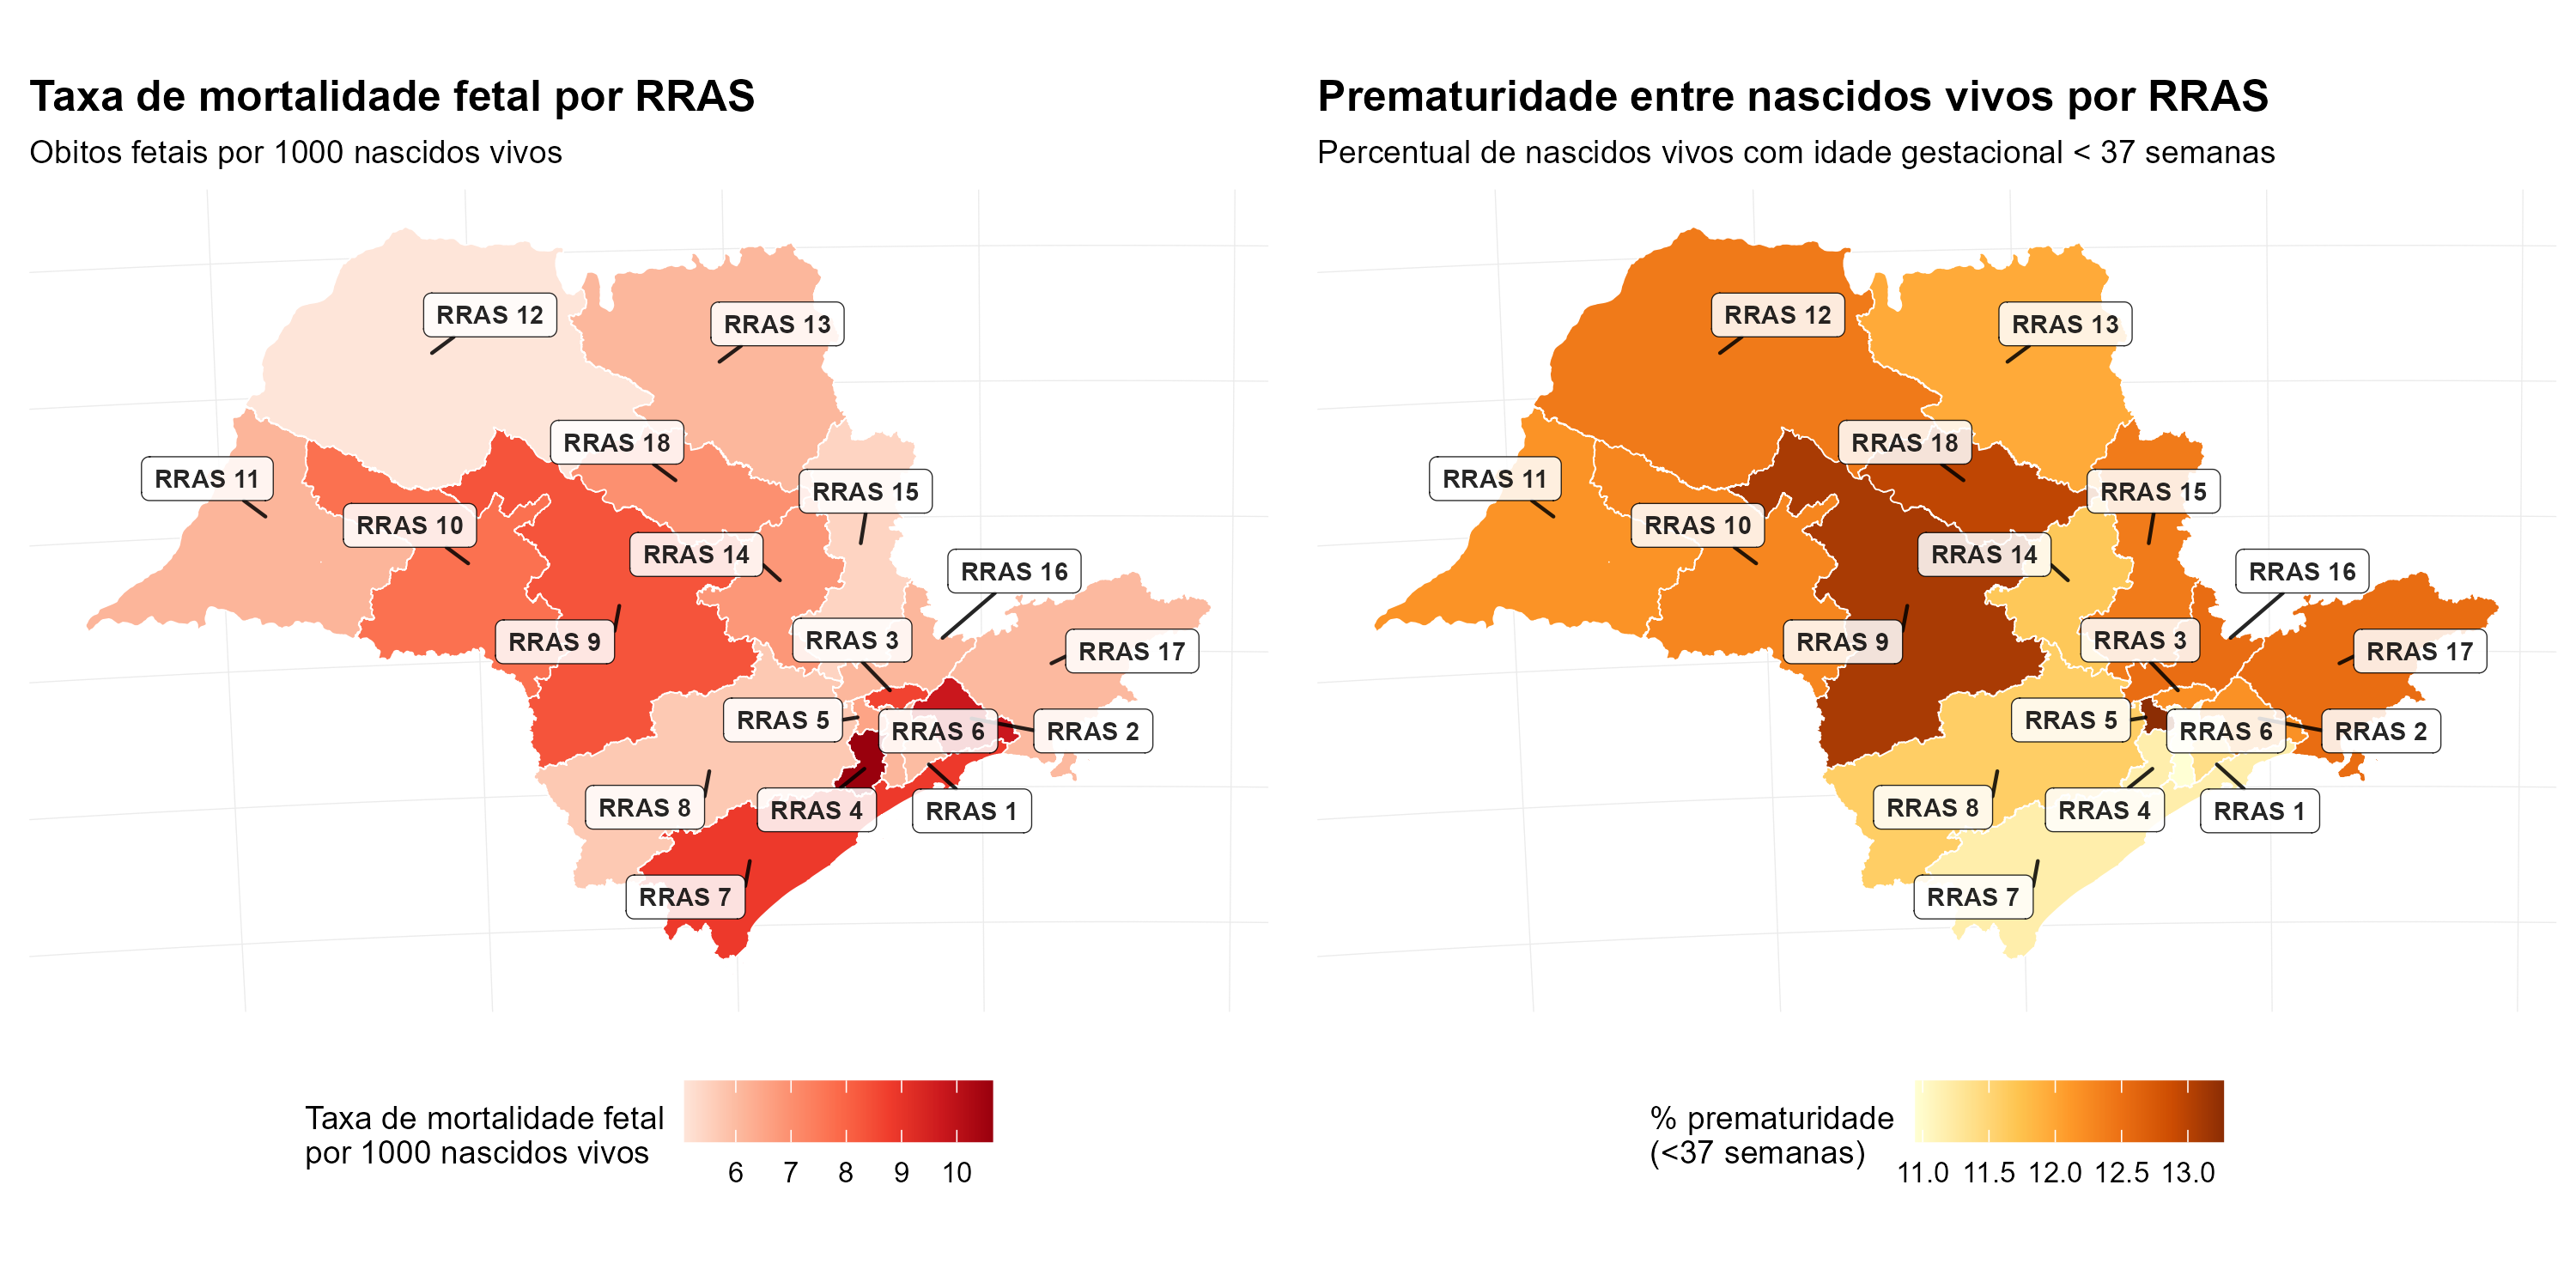
\includegraphics[width=0.9\linewidth]{figuras/mapas_RRAS_taxas_prematuridade.png}
  \fonte{Fonte: elaboração do autor.}
  \label{fig:mapas_RRAS_taxas_prematuridade}
\end{figure}

Em conjunto, os resultados por RRAS mostram heterogeneidade regional tanto nas
frequências absolutas quanto nas taxas. Essa variação reforça a importância de
considerar a RRAS como nível de agrupamento na modelagem, com inclusão de
fragilidade compartilhada e termo espacial, já que regiões com organização
assistencial e contexto territorial distintos podem apresentar comportamentos
também distintos no tempo até o parto.

\section{Resultados do modelo}
